\chapter{Testing}

\section{Test Plan}

\begin{landscape}
\subsection{Original Outline Plan}
\begin{center}
    \begin{tabular}{|p{2cm}|p{5cm}|p{5cm}|p{4cm}|}
        \hline

        \textbf{Test Series} & \textbf{Purpose of Test Series} & \textbf{Testing Strategy} & \textbf{Strategy Rationale}\\ \hline
	1. & Test the flow of control between the user interfaces & Top Down Testing & I Have chosen Top Down Testing Because the System begins with a main Interface then stems into different interfaces. \\ \hline
	2. & Test validation of data inputs & Bottom Up testing Testing &  Each input and output will be tested when they're developed\\ \hline
	3. & Test Data is stored in the correct location & White Box Testing & i am using White box testing because i will have to look into the database once the data is added \\ \hline
	4. & Test algorithms and SQL statements to ensure the output is correct & Black box testing & I am using Black Box Testing because i can see whether the algorithms work without having to look at the code and SQL Queries. \\ \hline
	5. & Test the system fulfils the specification & Acceptance testing & I have used acceptance testing because the test is to see if the system fulfils the specification. \\ \hline

    \end{tabular}
\end{center}
\end{landscape}
\subsection{Changes to Outline Plan}
	Some of my test series were quite brief and only tested for one variable. For example test series 3, ' Test Data is stored in the correct location' only tests whether the data is stored in the correct location. Because i am storing encrypted passwords, and data that must be in a specific format, such as dates, i have change this test series to: 'Test data is stored in the correct format and is in the correct storage location'. \par

 Looking at my original test plan, there are many aspects of my system in which i am not testing. One area which is not being tested is the emailing functionality. I need to test whether the emails are being sent to the correct email address, and that the contents of the email address are appropriate. For example i don't want the system to send an email to a user their account details, when i actually want to send them an email containing an invoice. Therefore i have added a test series to test the emailing functionality. \par

During the implementation process i added keyboard shortcuts to increase the speed of flow of control between the interfaces. In my original outline plan there were no test to see if these keyboard shortcuts work as they should. Therefore, i have added a new test series to test the functionalilty of the keyboard shortcuts. \par

Below is a table to show the changes i have made to the original outline plan created during the design phase. Any Test series that have been modified are highlighted in dark grey  and any new test series added have been highlighted in light grey.

\begin{landscape}
\begin{center}
    \begin{tabular}{|p{2cm}|p{5cm}|p{5cm}|p{4cm}|}
        \hline
	
	 \textbf{Test Series} & \textbf{Purpose of Test Series} & \textbf{Testing Strategy} & \textbf{Strategy Rationale}\\ \hline
	1. & Test the flow of control between the user interfaces & Top Down Testing & I Have chosen Top Down Testing Because the System begins with a main Interface then stems into different interfaces. \\ \hline
	2. & Test validation of data inputs & Bottom Up testing Testing &  Each input and output will be tested when they're developed\\ \hline
	\rowcolor{dark-grey} 3. & Test Data is stored in the correct location & White Box Testing & i am using White box testing because i will have to look into the database once the data is added \\ \hline
	\rowcolor{light-grey} 3. & Test Data is stored in the correct location and is in the correct format & White Box Testing & i am using White box testing because i will have to look into the database once the data is added \\ \hline
	4. & Test algorithms and SQL statements to ensure the output is correct & Black box testing & I am using Black Box Testing because i can see whether the algorithms work without having to look at the code and SQL Queries. \\ \hline
	\rowcolor{light-grey} 5. & Test that the email features work and that the contents of each email is appropriate & Black-Box Testing & I'm using black box testing because i can get the results from the test without having to look at the code.\\ \hline
	\rowcolor{light-grey} 6. & Test that each keyboard short-cut does what it should & Black-Box testing & I'm using black box testing because I can test this feature without having to look at the code from my system. \\ \hline
	7. & Test the system fulfils the specification & Acceptance testing & I have used acceptance testing because the test is to see if the system fulfils the specification. \\ \hline

    \end{tabular}
\end{center}
\end{landscape}
\subsection{Original Detailed Plan}

the table below shows my original test plan made during the design phase. Since the design phase i have implemented my system and made alterations to the features described during the design phase. Because of these changes made, i have removed some tests from my original test plan as they have become redundant due to the changes made during the implementation stage. Some tests have been removed because they require a few modifications to suit my system after the implementation stage, both the removed and modified tests are described in the 'Changes to Detailed Plan' section. 

\begin{flushleft}
\begin{longtable}{|p{1.5cm}|p{2.5cm}|p{2.5cm}|p{2cm}|p{2cm}|p{2cm}|p{2cm}|p{2cm}|}
        \hline
        \textbf{Test Series} & \textbf{Purpose of Test} & \textbf{Test Description} &  \textbf{Expected Result} & \textbf{Annotation Reference}\\ \hline
	1.01 & Test the Arrow button to see if it works successfully & The Arrow Button Should change to the Product Search Interface if log in details are correct & The Product Search Interface should be displayed &  \\ \hline
	1.02 & Test the keyboard short-cut assigned to the arrow button works successfully & The Keyboard Shortcut Should change to the Product Search Interface if log in details are correct &The Product Search Interface should be displayed &  \\ \hline
	1.03 & Test the Reset Password Here Link & When clicked the Link should change to the reset password interface  & The Reset Password Interface should be displayed &  \\ \hline
	1.04 & Test the Log Off button to see if it works successfully & Left mouse clicking the log off button should return back to the log in interface l & The Log in interface should be displayed &\\ \hline
	1.05 & Test to see if the Add new product option works successfully & The user should left click on the product tab then left click on the Add new product Option. &  The interface should change to the Add new product interface& \\ \hline
	1.06 & Test to see if the Delete Product button works & Clicking on the product tab then clicking on the delete product option & Interface should change to Delete a product interface& \\ \hline
	1.07 & Test to see if the manage stock button works successfully & Clicking on the Manage Stock button to see what the outcome is & The Stock Management interface should be displayed. & \\ \hline
	1.08 & Test to see if the Product restock button works & Clicking the Product restock button to see the result & The Stock management interface should be displayed. & \\ \hline
	1.09 & Test to see if the add a new member button works & The Add new member button should change to the Add new member interfacel & the Add new member interface should be displayed& \\ \hline
	1.10 & Testing to see what happens when remove member is clicked & left clicking the delete member button and recording outcome & the Remove a member interface should be displayed & \\ \hline
	1.11 & Test to see if the add a new employee button works & The Add new employee button should change to the Add new employee interface &  the Add new employee interface should be displayed& \\ \hline
	1.12 & Testing to see what happens when remove employee is clicked & left clicking the employee member button and recording outcome & the Remove a employee interface should be displayed & \\ \hline
	2.01 & Testing valid characters and range of Product Name & entering a range of different characters to see which ones are valid & The string Test should be accepted however, the characters `123' and `@+' should not be accepted as they are integers and special characters & \\ \hline
	2.02 & testing to see which file types are valid for Product Image & entering a range of file types to see which are valid & The only accepted file types should be .jpg and .png. No other file extensions should be valid. & \\ \hline
	2.03 & testing to see which file types are valid for Product Image & entering an erroneous file type to see if its accepted &  Should not be accepted as a valid image file & \\ \hline
	2.04 & Testing to see which characters are valid in Price & entering a range of characters into price to see which are accepted &  None of the characters should be accepted because a price cannot contain letters or special characters & \\ \hline
	2.05 & Testing to see which characters are valid in Stock & entering a range of characters into the stock field and seeing which are valid  & The Integers should be accepted by the system& \\ \hline
	2.06 & Testing to see which characters are valid in Stock & entering a range of characters into the stock field and seeing which are valid  & The letters `test' and special characters `@+' should be invalid because as the stock is only defined by integers.& \\ \hline
	2.07 & Testing to see which characters are valid in Name & Entering a range of characters into name and seeing which ones are valid  & Only the letters `test' should be valid as a name cannot contain integers or special characters.& \\ \hline
	2.08 & Testing to see which characters are valid in Name & Entering a range of characters into name and seeing which ones are valid &  The above text should not be valid as it contain number sand special characters, a name can only contain letters.& \\ \hline
	2.09 & seeing which characters are valid in email & Entering Erroneous data to see if it is accepted into the database  & This string should not be accepted as a legitimate email because it does not contain the ``.com''& \\ \hline
	2.10 & seeing which characters are valid in email & Entering Erroneous data to see if it is accepted into the database  &  This string should not be accepted as a legitimate email because it does not contain the @'' & \\ \hline
	2.11 & seeing which characters are valid in email & Entering a valid email to see if it is accepted  &  Bob@ Email.com should be accepted. This is because it contains both the @ symbol and is followed by .com & \\ \hline
	2.12 & testing for validation in telephone number & Entering an 11 digit telephone number  & this telephone number contains exactly 11 digits therefore it should be valid & \\ \hline
	2.13 & testing for validation in telephone number & Entering a 3 Digit telephone Number &  `999' is too short and should not be accepted as a telephone number& \\ \hline
	2.14 & testing for validation in telephone number & Entering a telephone number thats longer than the boundary & This number should not be accepted because it is too long & \\ \hline
	2.15 & testing for validation in telephone number &Entering an 11 digit number to see if it is outside the boundary  & this number should be accepted because it is 11 digits long & \\ \hline
	2.16 & testing for validation in telephone number & Entering a 12 digit number to see if it is outside the boundary & this number should not be accepted because it is 12 digits long & \\ \hline
	3.01 & Product Name is added to the database successfully & Adding a Product to the database and make sure the product Name has been added successfully & The ProductName should be Pedigree Chum and the rest of the data should be stored in the Product Table & \\ \hline
	3.02 & The correct Product image is assigned to the right Product & Adding a Product to the database and make sure the correct Product Image is assigned to the Product & The ProductImage entered should be assigned to the Product Entered. & \\ \hline
	3.03 & Ensuring all product data is stored in the product table & Entering a product then ensuring all of its data is input into the Product table  & The ProductName should be Dog Food and the rest of the data should be stored in the Product Table & \\ \hline
	3.04 & Ensuring The Postcode the User enters is stored in the correct format  & To prevent any errors when trying to search for the postcode later on  & The Postcode has three numbers and letters then the space, then four numbers and letters. & \\ \hline
	3.05 & Ensuring The Postcode the User enters is stored in the correct format  & To prevent any errors when trying to search for the postcode later on  & The postcode does not contain a space between the two parts of the postcode, therefore it should not be accepted in the database. & \\ \hline
	3.06 & Ensuring all member data is stored in the member table & Entering a member then ensuring all of its data is input into the member table  & The MemberName should be Bruce Wayne  and the rest of the data should be stored in the Member Table & \\ \hline
	3.07 & Ensuring the Employees password is set to `Password' When the account is first created & Adding an Employee then using the password `password' to enter the account. & The password should be accepted and the employee should be taken to the change password screen& \\ \hline
	3.08 & Ensuring the reset password email is sent to the correct email address. & Changing the password for the employee and ensuring the password reset email goes to their email address. & The employee should log on the email address associated with their Employee Account and the email should be in their in-box.& \\ \hline
	3.09 & Ensuring all Employee data is stored in the Employee table & Entering a employee then ensuring all of its data is input into the Employee table & The EmployeeName should be Clark Kent and the rest of the data should be stored in the Employee Table & \\ \hline
	4.01 & Ensuring the product table is created properly & Creating the product table and adding a product to ensure its working properly & The Table should be created and the product Dog Food should be added successfully. Al the data should be in its corresponding column & \\ \hline
	4.02 & Editing a Product within the database &  change some data assigned to a specific product and see if the data has successfully changed within the database. & The Product Name of the product the user wants to edit should be changed to Cat Nibbles and the data should successfully update within the database. & \\ \hline
	4.03 & Editing a Member within the database &  change some data assigned to a specific member and see if the data has successfully changed within the database. &  The Member Title should be changed to ``sgt.'' and the data should successfully update within the database.  & \\ \hline
	4.04 & Editing a Employee within the database &  changing the email address associated with a specific employee & The Employees email address should have changed and the data should successfully update within the database& \\ \hline
	4.05 & Deleting a product from the database &  Entering a ProductID to delete then seeing if it was deleted successfully & The product database should be viewed, then a productID from a Product should be taken from the database should. this ProductID should be entered into the SQL statement. If the statement worked, the product should no longer be in the database & \\ \hline
	4.06 & Deleting a Member from the database &  Entering a MemberID to delete then seeing if it was deleted successfully & The Member with the MemberID entered by the user should now be removed from the Member Table within the database. & \\ \hline
	4.07 & Deleting an Employee from the database &  Entering an EmployeeID to delete then seeing if it was deleted successfully & The Employee with the EmployeeID entered by the user should now be removed from the Employee Table within the database & \\ \hline
	4.08 & Trying to delete the Administrator account  & Entering the EmployeeID of the My Client (The Administrator) and seeing if it can be removed from the system. & The Account should not be allowed to be deleted from the system as the will leave no administrative account on the system & \\ \hline
	5.01 & Verify the program fulfils the specification & Run the program, testing the different aspects to ensure it meets the specification  &system fulfils the specification & \\ \hline
\end{longtable}
\end{flushleft}

\subsection{Changes to Detailed Plan}

Since i created my original outline plan during the design phase, i have add two new test plans. This means i shall now need to include more tests to my detailed plan to test each feature in the new test series. As stated before, i have removed some test series as since the implementation stage, i have made a few modifications to my system. The tests in which i have removed have been highlighted in dark grey. Any tests that i have added have been highlighted in light grey.

\begin{flushleft}
\begin{longtable}{|p{1cm}|p{2.5cm}|p{2.5cm}|p{2cm}|p{2cm}|}
        \hline
        \textbf{Test Series} & \textbf{Purpose of Test} & \textbf{Test Description} &  \textbf{Expected Result} & \textbf{Annotation Reference}\\ \hline
	\rowcolor{dark-grey}1.01 & Test the Arrow button to see if it works successfully & The Arrow Button Should change to the Product Search Interface if log in details are correct & The Product Search Interface should be displayed &  \\ \hline
	\rowcolor{light-grey}1.01 & Test to see if the Enter Button Functions as it should & Clicking the Enter button After Entering Log in Details & If the Log-in information matches an account in the system, the user should get taken to the create an order window, otherwise a message should be displayed saying that the details are not valid &  Page:\pageref{fig:101-1}  \newline Figure:\ref{fig:101-1}  \newline  \newline Page:\pageref{fig:101-2}  \newline Figure:\ref{fig:101-2} \newline  \newline Page:\pageref{fig:101-3}  \newline Figure:\ref{fig:101-3}\\ \hline
	\rowcolor{dark-grey}1.02 & Test the keyboard short-cut assigned to the arrow button works successfully & The Keyboard Short-cut Should change to the Product Search Interface if log in details are correct &The Product Search Interface should be displayed &  \\ \hline
	1.02 & Test the Reset Password Here Link & When clicked the Link should change to the reset password interface  & The Reset Password Interface should be displayed &  \newline Figure:\ref{fig:102-1} \newline  \newline  Page:\pageref{fig:102-2}  \newline Figure:\ref{fig:102-2}\\ \hline
	1.03 & Test the Log Off button to see if it works successfully & Left mouse clicking the log off button should return back to the log in interface l & The Log in interface should be displayed &  Page:\pageref{fig:103-1}  \newline Figure:\ref{fig:103-1} \newline  \newline  Page:\pageref{fig:103-2}  \newline Figure:\ref{fig:103-2}  \newline  \newline  Page:\pageref{fig:103-3}  \newline Figure:\ref{fig:103-3}\\ \hline
	1.04 & Test to see if the Add new product option works successfully & The User should click on the Product Menu in the Menu-bar and then click on Add Product &  The interface should change to the Add new product interface& Page:\pageref{fig:104-1}  \newline Figure:\ref{fig:104-1} \newline  \newline Page:\pageref{fig:104-2}  \newline Figure:\ref{fig:104-2}\\ \hline
	1.05 & Test to see if the Delete Product button works & Clicking on the product tab then clicking on the delete product option & Interface should change to Delete a product interface&  Page:\pageref{fig:105-1}  \newline Figure:\ref{fig:105-1} \newline  \newline Page:\pageref{fig:105-2}  \newline Figure:\ref{fig:105-2}\\ \hline
	1.06 & Test to see if the manage stock button works successfully & Clicking on the Manage Stock button to see what the outcome is & The Stock Management interface should be displayed. &  Page:\pageref{fig:106-1}  \newline Figure:\ref{fig:106-1} \newline  \newline Page:\pageref{fig:106-2}  \newline Figure:\ref{fig:106-2}\\ \hline
	\rowcolor{dark-grey}1.07 & Test to see if the Product restock button works & Clicking the Product restock button to see the result & The Stock management interface should be displayed. & \\ \hline
	1.07 & Test to see if the add a new member button works & The Add new member button should change to the Add new member interface & the Add new member interface should be displayed&  Page:\pageref{fig:107-1}  \newline Figure:\ref{fig:107-1} \newline  \newline Page:\pageref{fig:107-2}  \newline Figure:\ref{fig:107-2}\\ \hline
	1.08 & Testing to see what happens when remove member is clicked & left clicking the delete member button and recording outcome & the Remove a member interface should be displayed &  Page:\pageref{fig:108-1}  \newline Figure:\ref{fig:108-1} \newline  \newline Page:\pageref{fig:108-2}  \newline Figure:\ref{fig:108-2}\\ \hline
	1.09 & Test to see if the add a new employee button works & The Add new employee button should change to the Add new employee interface &  the Add new employee interface should be displayed&   Page:\pageref{fig:109-1}  \newline Figure:\ref{fig:109-1} \newline  \newline Page:\pageref{fig:109-2}  \newline Figure:\ref{fig:109-2} \newline  \newline  Page:\pageref{fig:109-3}  \newline Figure:\ref{fig:109-3}\\ \hline
	1.10 & Testing to see what happens when remove employee is clicked & left clicking the employee member button and recording outcome & the Remove a employee interface should be displayed &  Page:\pageref{fig:110-1}  \newline Figure:\ref{fig:110-1}  \newline  \newline Page:\pageref{fig:110-2}  \newline Figure:\ref{fig:110-2}\\ \hline
	2.01 & Testing valid characters and range of Product Name & entering a range of different characters to see which ones are valid & The Product name should allow a combination of letters and numbers, no special characters & Page:\pageref{fig:201-1}  \newline Figure:\ref{fig:201-1}  \newline  \newline Page:\pageref{fig:201-2}  \newline Figure:\ref{fig:201-2}\\ \hline
	2.02 & testing to see which file types are valid for Product Image & entering a range of file types to see which are valid & The system should only accept .jpg or .png file types &  Page:\pageref{fig:202-1}  \newline Figure:\ref{fig:202-1} \newline  \newline   Page:\pageref{fig:202-2}  \newline Figure:\ref{fig:202-2} \\ \hline
	\rowcolor{dark-grey}2.03 & testing to see which file types are valid for Product Image & entering an erroneous file type to see if its accepted &  Should not be accepted as a valid image file & \\ \hline
	2.03 & Testing to see which characters are valid in Price & entering a range of characters into price to see which are accepted &  None of the characters should be accepted because a price cannot contain letters or special characters &  Page:\pageref{fig:203-1}  \newline Figure:\ref{fig:203-1}\newline  \newline Page:\pageref{fig:203-3}  \newline Figure:\ref{fig:203-3}  \newline  \newline Page:\pageref{fig:203-2}  \newline Figure:\ref{fig:203-2}  \\ \hline
	2.04 & Testing to see which characters are valid in Stock & entering a range of characters into the stock field and seeing which are valid  & The Integers should be accepted by the system & Page:\pageref{fig:204-1}  \newline Figure:\ref{fig:204-1}    \newline  \newline Page:\pageref{fig:204-2}  \newline Figure:\ref{fig:204-2}  \newline  \newline Page:\pageref{fig:204-3}  \newline Figure:\ref{fig:204-3}  \newline  \newline Page:\pageref{fig:204-4}  \newline Figure:\ref{fig:204-4} \\ \hline
	\rowcolor{dark-grey}2.06 & Testing to see which characters are valid in Stock & entering a range of characters into the stock field and seeing which are valid  & The letters `test' and special characters `@+' should be invalid because as the stock is only defined by integers. & \\ \hline
	\rowcolor{dark-grey}2.07 & Testing to see which characters are valid in Name & Entering a range of characters into name and seeing which ones are valid  & Only the letters `test' should be valid as a name cannot contain integers or special characters.& \\ \hline
	2.05 & Testing to see which characters are valid in Member Name & Entering a range of characters into name and seeing which ones are valid &  The text should Only accept letters. it should not accept numbers or special characters& Page:\pageref{fig:205-1}  \newline Figure:\ref{fig:205-1} \newline  \newline Page:\pageref{fig:205-2}  \newline Figure:\ref{fig:205-2}  \newline  \newline Page:\pageref{fig:205-3}  \newline Figure:\ref{fig:205-3} \newline  \newline Page:\pageref{fig:205-4}  \newline Figure:\ref{fig:205-4}  \newline  \newline   Page:\pageref{fig:205-5}  \newline Figure:\ref{fig:205-5} \\ \hline
	\rowcolor{dark-grey}2.10 & seeing which characters are valid in email & Entering Erroneous data to see if it is accepted into the database  & This string should not be accepted as a legitimate & \\ \hline
	\rowcolor{dark-grey}2.11 & seeing which characters are valid in Member email & Entering a valid email to see if it is accepted  &  Bob@ Email.com should be accepted. This is because it contains both the @ symbol and is followed by .com & \\ \hline
	\rowcolor{light-grey}2.06 & seeing which characters are valid in Member email & Entering a range of different characters into the member email field &  All characters should be valid in the member email field. &  Page:\pageref{fig:206-1}  \newline Figure:\ref{fig:206-1} \newline  \newline Page:\pageref{fig:206-2}  \newline Figure:\ref{fig:206-2} \newline  \newline  Page:\pageref{fig:206-3}  \newline Figure:\ref{fig:206-3} \\ \hline
	\rowcolor{dark-grey}2.12 & testing for validation in telephone number & Entering an 11 digit telephone number & this telephone number contains exactly 11 digits therefore it should be valid &  \\ \hline
	\rowcolor{dark-grey}2.14 & testing for validation in telephone number & Entering a telephone number that's longer than the boundary & This number should not be accepted because it is too long & \\ \hline
	\rowcolor{light-grey}2.07 & testing for validation in the postcode & Entering a range of different characters into the postcode field & only letters and numbers should be allowed into this field, special characters should not.All letters should automatically be capitalized&  Page:\pageref{fig:207-1}  \newline Figure:\ref{fig:207-1} \newline  \newline  Page:\pageref{fig:207-2}  \newline Figure:\ref{fig:207-2}  \newline  \newline Page:\pageref{fig:207-3}  \newline Figure:\ref{fig:207-3}  \\ \hline
	\rowcolor{light-grey}2.08 & Testing to see If the find postcode button works & Entering a postcode with and without a space between the two parts to see if it is found &The Postcode should be found even if the space between the two parts is or is not present.& Page:\pageref{fig:208-1}  \newline Figure:\ref{fig:208-1} \newline \newline Page:\pageref{fig:208-2}  \newline Figure:\ref{fig:208-2} \\ \hline
	\rowcolor{light-grey}2.09 & testing which values can be entered into the house number field & Entering a range of different characters into the house number field & only numbers should be allowed in this field, letters and special characters should not be allowed &  \\ \hline
	\rowcolor{light-grey}2.10 & Testing to see which characters are able to be entered into the Telephone number field & Entering a range of different characters into the telephone number field & only numbers should be allowed in this field, letters and special characters should not be allowed & \\ \hline
	\rowcolor{dark-grey}3.01 & Product Name is added to the database successfully & Adding a Product to the database and make sure the product Name has been added successfully & The ProductName should be Pedigree Chum and the rest of the data should be stored in the Product Table & \\ \hline
	\rowcolor{light-grey}3.01 & Product Name is added to the database successfully & Typing a name into the ProductName field and then adding the product to the database & The product name stored in the database should be the same as the text in the Product Name field.& Page:\pageref{fig:301-1}  \newline Figure:\ref{fig:301-1} \newline \newline  \\ \hline
	3.02 & The correct Product image is assigned to the right Product & Adding a Product to the database and make sure the correct Product Image is assigned to the Product & The ProductImage entered should be assigned to the Product Entered. & \\ \hline
	\rowcolor{dark-grey}3.03 & Ensuring all product data is stored in the product table & Entering a product then ensuring all of its data is input into the Product table  & The ProductName should be Dog Food and the rest of the data should be stored in the Product Table & \\ \hline
	\rowcolor{light-grey}3.03 & Ensuring all product data is stored in the product table & Entering a value into every data field for the product and checking the Product Table to ensure all the data is stored under the correct heading.  & The Product Name stored in the database should be the same as the Product Name entered by the user, the Price stored in the database should be the same as the price entered by the user, ect\ldots &  Page:\pageref{fig:303-1}  \newline Figure:\ref{fig:303-1} \\ \hline
	\rowcolor{dark-grey}3.04 & Ensuring The Postcode the User enters is stored in the correct format  & To prevent any errors when trying to search for the postcode later on  & The Postcode has three numbers and letters then the space, then four numbers and letters. & \\ \hline
	\rowcolor{light-grey}3.04 & Ensuring The Postcode the User enters is stored in the correct format  & Entering a postcode into the postcode field and only adding the Member to the database if the Postcode follows the regular expression. &if the postcode entered by the user matches the regular expression, then it is a valid postcode. Only if it matches, should it be allowed to be added to the Member Table within the database.&  Page:\pageref{fig:304-1}  \newline Figure:\ref{fig:304-1} \\ \hline
	\rowcolor{dark-grey}3.05 & Ensuring The Postcode the User enters is stored in the correct format  & To prevent any errors when trying to search for the postcode later on  & The postcode does not contain a space between the two parts of the postcode, therefore it should not be accepted in the database. & \\ \hline
	\rowcolor{light-grey}3.05 & Ensuring all member data is stored in the member table & Entering a member then ensuring all of its data is input into the member table  & The MemberName should be Bruce Wayne  and the rest of the data should be stored in the Member Table & Page:\pageref{fig:305-1}  \newline Figure:\ref{fig:305-1}\\ \hline
	\rowcolor{light-grey}3.06 & Ensuring the member data entered by the user is stored under the correct headings in the Member Table. & Entering a value into each data field for the Member then adding them to the database. & Each value entered by the user shoudl be stored under the correct heading in the Members Table within the database. &  Page:\pageref{fig:306-1}  \newline Figure:\ref{fig:306-1} \newline \newline  Page:\pageref{fig:306-2}  \newline Figure:\ref{fig:306-2} \\ \hline
	\rowcolor{dark-grey}3.07 & Ensuring the Employees password is set to `Password' When the account is first created & Adding an Employee then using the password `password' to enter the account. & The password should be accepted and the employee should be taken to the change password screen& \\ \hline
	\rowcolor{light-grey}3.07 & Ensuring the Employees password is set to `Password' When the account is first created & Creating an employee account and checking the database to see what the Employee Password is. & Adding an Employee to the database and checking that the password stored in the database is `password'. That employee should then be able to log in with their user-name and the password `password'. & \\ \hline
	\rowcolor{dark-grey}3.08 & Ensuring the reset password email is sent to the correct email address. & Changing the password for the employee and ensuring the password reset email goes to their email address. & The employee should log on the email address associated with their Employee Account and the email should be in their in-box.& \\ \hline
	\rowcolor{dark-grey}3.09 & Ensuring all Employee data is stored in the Employee table & Entering a employee then ensuring all of its data is input into the Employee table & The EmployeeName should be Clark Kent and the rest of the data should be stored in the Employee Table & \\ \hline
	\rowcolor{light-grey}3.08 & Ensuring that the stock changed by the user, matches the stock in the database. & Finding a product in the Manage Stock window and changing the stock in one of the locations and saving the Product. & Once the User has changed the stock and saved the changes, the stock within the database should have changed accordingly. & Page:\pageref{fig:308-1}  \newline Figure:\ref{fig:308-1} \newline \newline  Page:\pageref{fig:308-2}  \newline Figure:\ref{fig:308-2} \\ \hline
	\rowcolor{dark-grey}4.01 & Ensuring the product table is created properly & Creating the product table and adding a product to ensure its working properly & The Table should be created and the product Dog Food should be added successfully. Al the data should be in its corresponding column & \\ \hline
	\rowcolor{light-grey}4.01 & Ensuring the product table is created properly & Creating the product table and adding a product to ensure its working properly & There should be a new table called Product and the Table should contain a Product with a name, price, image path ,product stock, a category and a size.& \\ \hline
	\rowcolor{dark-grey}4.02 & Editing a Product within the database &  change some data assigned to a specific product and see if the data has successfully changed within the database. & The Product Name of the product the user wants to edit should be changed to Cat Nibbles and the data should successfully update within the database. & \\ \hline
	\rowcolor{light-grey}4.02 & Editing a Product within the database & Find an existing product within the database, change some of the existing data then save it in the database. & Any data in which the user has changed should have changed within the database after they have saved it. & Page:\pageref{fig:402-1}  \newline Figure:\ref{fig:402-1} \newline \newline  Page:\pageref{fig:402-2}  \newline Figure:\ref{fig:402-2} \\ \hline
	\rowcolor{dark-grey}4.03 & Editing a Member within the database &  change some data assigned to a specific member and see if the data has successfully changed within the database. &  The Member Title should be changed to ``Sgt.'' and the data should successfully update within the database.  & \\ \hline
	\rowcolor{light-grey}4.03 & Editing a Member within the database & Find an existing member within the database and change some some of the data, save the Member and see if the changes have been made within the database. &  Any changes made by the member should have been changed within the database if the user saved the changes.& Page:\pageref{fig:403-1}  \newline Figure:\ref{fig:403-1} \newline \newline  Page:\pageref{fig:403-2}  \newline Figure:\ref{fig:403-2} \\ \hline
	\rowcolor{dark-grey}4.04 & Editing a Employee within the database &  changing the email address associated with a specific employee & The Employees email address should have changed and the data should successfully update within the database& \\ \hline
	\rowcolor{light-grey}4.04 & Editing an Employee within the database &  Finding an existing employee within the database and change some of the data fields, then save the employee & The Employee data should have changed within the database and the Employee User-name should have changed accordingly if the employees first or last name was changed.&  Page:\pageref{fig:404-1}  \newline Figure:\ref{fig:404-1} \newline \newline  Page:\pageref{fig:404-2}  \newline Figure:\ref{fig:404-2}\\ \hline
	4.05 & Deleting a product from the database &  Entering a ProductID to delete then seeing if it was deleted successfully & The product database should be viewed, then a ProductID from a Product should be taken from the database should. this ProductID should be entered into the SQL statement. If the statement worked, the product should no longer be in the database &  Page:\pageref{fig:405-1}  \newline Figure:\ref{fig:405-1} \newline \newline  Page:\pageref{fig:405-2}  \newline Figure:\ref{fig:405-2} \\ \hline
	4.06 & Deleting a Member from the database &  Entering a MemberID to delete then seeing if it was deleted successfully & The Member with the MemberID entered by the user, should now be removed from the Member Table within the database. &  Page:\pageref{fig:406-1}  \newline Figure:\ref{fig:406-1} \newline \newline  Page:\pageref{fig:406-2}  \newline Figure:\ref{fig:406-2}\\ \hline
	4.07 & Deleting an Employee from the database &  Entering an EmployeeID to delete then seeing if it was deleted successfully & The Employee with the EmployeeID entered by the user should now be removed from the Employee Table within the database & Page:\pageref{fig:407-1}  \newline Figure:\ref{fig:407-1} \newline \newline  Page:\pageref{fig:407-2}  \newline Figure:\ref{fig:407-2} \\ \hline
	4.08 & Trying to delete the Administrator account  & Entering the EmployeeID of the My Client (The Administrator) and seeing if it can be removed from the system. & The Account should not be allowed to be deleted from the system as this will leave no administrative account on the system & Page:\pageref{fig:408-1}  \newline Figure:\ref{fig:408-1}\\ \hline
	\rowcolor{light-grey} 5.01 & Testing to see if the gmail account the emails being sent from are valid & Entering a gmail address and password and trying to send an email from the account. &If the account details are not correct, the system should return an error message to the user that the account details do not match. otherwise, the user should be told that the email has been sent. & Page:\pageref{fig:501-1}  \newline Figure:\ref{fig:501-1} \newline \newline  Page:\pageref{fig:501-2}  \newline Figure:\ref{fig:501-2}  \newline \newline  Page:\pageref{fig:501-3}  \newline Figure:\ref{fig:501-3}\\ \hline
	\rowcolor{light-grey} 5.02 & If the user wants to change their password, a code is emailed to them, this test is to test the functionality of this email. & The user clicks on the Change password option under the options menu, once clicked the email is sent to the employees email address. & An email is sent to the email address associated to that employees account, The email should contain a 4 digit code and some text informing the employee what the code is for. &  Page:\pageref{fig:502-1}  \newline Figure:\ref{fig:502-1} \newline \newline  Page:\pageref{fig:502-2}  \newline Figure:\ref{fig:502-2} \\ \hline
	\rowcolor{light-grey} 5.03 & Testing to see if the Invoice email is sent in HTML and has an appropriate subject to the email & Once an order has been created, the employee can email the invoice to a customer. The Employee enters the customers email address and clicks the save invoice button. Here email email is automatically sent. & When opened, the invoice  be displayed as a HTML document. The invoice in the email should match the invoice that was sent to the email. &\\ \hline
	\rowcolor{light-grey} 5.04 & Testing To see if the emails have an appropriate subject & Send an email using one of the methods from the previous three tests and checking that the email has an Appropriate subject & If the email sent contained an invoice for a customer, The subject of the email should inform the user that the contents of the email contains an invoice. & Page:\pageref{fig:504-1}  \newline Figure:\ref{fig:504-1}\\ \hline
	\rowcolor{light-grey} 6.01 & Test the Log Off short-cut to see if it works successfully & Pressing the `Escape' button on the keyboard when a user is logged in. to see if they get logged out & The user should be provided with a yes or no confirmation window as to whether they're sure they want to log off.  &  Page:\pageref{fig:601-1}  \newline Figure:\ref{fig:601-1}\\ \hline
	\rowcolor{light-grey} 6.02 & Test the keyboard short-cut assigned to the Enter button works successfully & Pressing `Enter' on the keyboard once the user has entered their log in details &  When the `Enter' button is pressed, if the Log-in information matches an account in the system, the user should get taken to the create an order window, otherwise a message should be displayed saying that the details are not valid& \\ \hline
	\rowcolor{light-grey} 6.03 & Testing the Search Window short-cut works appropriately &Once the user has logged in, pressing the `CTRL'  and `F' button on the keyboard  at the same time. & When `CTRL+F' are pressed the search window should open&  Page:\pageref{fig:603-1}  \newline Figure:\ref{fig:603-1} \\ \hline
	\rowcolor{light-grey} 6.04 & Testing the save product, member and employee short-cuts work appropriately & when either adding removing or editing a product, member or employee, the user can should press the `CTRL' and `S' buttons on the keyboard simultaneously & When CTRL+S are pressed simultaneously, the user should be displayed with a confirmation window whether they're sure they want to add edit or delete.&  Page:\pageref{fig:604-1}  \newline Figure:\ref{fig:604-1} \newline \newline   Page:  \pageref{fig:604-2}  \newline Figure:\ref{fig:604-2} \newline \newline Page:\pageref{fig:604-3}  \newline Figure:\ref{fig:604-3} \newline \newline Page:\pageref{fig:604-4}  \newline Figure:\ref{fig:604-4}  \newline \newline   Page:\pageref{fig:604-5}  \newline Figure:\ref{fig:604-5} \newline \newline   Page:  \pageref{fig:604-6}  \newline Figure:\ref{fig:604-6} \newline \newline Page:\pageref{fig:604-7}  \newline Figure:\ref{fig:604-7} \newline \newline Page:\pageref{fig:604-8}  \newline Figure:\ref{fig:604-8} \newline \newline   Page:  \pageref{fig:604-9}  \newline Figure:\ref{fig:604-9} \\ \hline
	\rowcolor{light-grey} 6.05 & Testing the Enter Short-cut once the user has logged in & If the user is not logged in the Enter button is used as a short-cut to log in. Once logged in, the Enter button on the keyboard is a short-cut to close all pop-up windows, or confirm the `Yes' choice on all confirmation windows. & If a Pop up window is displayed to the user and the only button they can click is an `OK' button. The `Enter' short-cut should close the window. If the user is presented with a confirmation with a `Yes' or `No' decision, pressing the `Enter' button on the keyboard should choose the `Yes' option. &  Page:\pageref{fig:605-1}  \newline Figure:\ref{fig:605-1} \\ \hline
	\rowcolor{light-grey} 6.06 & Testing the right click short-cuts in the Search window. & In the search Window the user right clicks a product, employee or member. Once right clicked a menu is displayed depending on if a product member or employee has been right clicked. & Clicking on one of the options in the menu should take the user to the relevant page.& Page:\pageref{fig:606-1}  \newline Figure:\ref{fig:606-1} \newline \newline Page:\pageref{fig:606-2}  \newline Figure:\ref{fig:606-2} \newline \newline  Page:\pageref{fig:606-3}  \newline Figure:\ref{fig:606-3} \\ \hline
	\rowcolor{light-grey} 6.07 & Testing the CTRL+P short-cut & Once Logged in, Pressing the `CTRL' and P keyboard buttons simultaneously & The user should be taken to the Adding Product Page& \\ \hline
	\rowcolor{light-grey} 6.08 & Testing the CTRL+M short-cut & Once Logged in, Pressing the `CTRL' and M keyboard buttons simultaneously & The user should be taken to the Adding Member Page& \\ \hline
	\rowcolor{light-grey} 6.09 & Testing the CTRL+E short-cut & Once Logged in, Pressing the `CTRL' and E keyboard buttons simultaneously & The user should be taken to the Adding Employee Page& \\ \hline
	\rowcolor{light-grey} 6.10 & Testing the CTRL+O short-cut & Once Logged in, Pressing the `CTRL' and O keyboard buttons simultaneously & The user should be taken to the Create Order Page& \\ \hline
	7.01 & Verify the program fulfils the specification & Run the program, testing the different aspects to ensure it meets the specification  & system fulfils the specification & \\ \hline
\end{longtable}
\end{flushleft}

\pagebreak

\section{Test Data}

\subsection{Original Test Data}
	\begin{flushleft}
    \begin{longtable}{|p{1.5cm}|p{2.5cm}|p{2cm}|p{4.5cm}|}
        \hline
        \textbf{Test Series} & \textbf{Test Data} & \textbf{Test Data Type (Normal/ Erroneous/ Boundary)} &  \textbf{Justification for Choice of test data}\\ \hline
	1.01 & Click the arrow button & Normal & The Product Search Interface should be displayed  \\ \hline
	1.02 & Press the Keyboard Short-cut after legitimate log in details are entered &  Normal & The Product Search Interface should be displayed \\ \hline
	1.03 & Left mouse click on the Reset Password Link &  Normal & The Reset Password Interface should be displayed  \\ \hline
	1.04 & Left mouse click Log off button &  Normal & The Log in interface should be displayed  \\ \hline
	1.05 & Left click Add new product button &  Normal &  The interface should change to the Add new product interface \\ \hline
	1.06 &  Left mouse click Delete a product button &  Normal & Interface should change to Delete a product interface \\ \hline
	1.07 & The Manage Product button, under the Stock tab should be left clicked &  Normal & The Stock Management interface should be displayed.  \\ \hline
	1.08 &  left clicking the Stock tab then left clicking the Product restock tab &  Normal & The Stock management interface should be displayed.  \\ \hline
	1.09 &  Left clicking the add new member button under the member tab &  Normal & the Add new member interface should be displayed \\ \hline
	1.10 & Left clicking remove a member under the member tab & Normal & the Remove a member interface should be displayed  \\ \hline
	1.11 & Left clicking the add new employee button under the employee tab &  Normal & the Add new employee interface should be displayed \\ \hline
	1.12 & Left clicking remove a employee under the employee tab & Normal & the Remove a employee interface should be displayed  \\ \hline
	2.01 & Test123@+ & Normal & The string Test should be accepted however, the characters `123' and `@+' should not be accepted as they are integers and special characters  \\ \hline
	2.02 &  test.jpg, test.bnp, test.txt, test.png, test.gif, test.doc, test.pdf & Normal & The only accepted file types should be .jpg and .png. No other file extensions should be valid.  \\ \hline
	2.03 &  test.doc & Erroneous &  Should not be accepted as a valid image file  \\ \hline
	2.04 &  test@+ & Erroneous  &  None of the characters should be accepted because a price cannot contain letters or special characters  \\ \hline
	2.05 &  11  & Normal & The Integers should be accepted by the system \\ \hline
	2.06 &  test@+ & Erroneous & The letters `test' and special characters `@+' should be invalid because as the stock is only defined by integers. \\ \hline
	2.07 &  Matthew & Normal & Only the letters `test' should be valid as a name cannot contain integers or special characters. \\ \hline
	2.08 &  =John34 & Erroneous & The above text should not be valid as it contain number sand special characters, a name can only contain letters. \\ \hline
	2.09 &   Bob@ email  & Erroneous & This string should not be accepted as a legitimate email because it does not contain the ``.com'' \\ \hline
	2.10 &  Bob.com& Erroneous &  This string should not be accepted as a legitimate email because it does not contain the @'' \\ \hline
	2.11 &  Bob@ email.com & Normal &  Bob@ Email.com should be accepted. This is because it contains both the @ symbol and is followed by .com \\ \hline
	2.12 &  01234567890 & Normal & this telephone number contains exactly 11 digits therefore it should be valid \\ \hline
	2.13 &  999& Erroneous &  `999' is too short and should not be accepted as a telephone number \\ \hline
	2.14 &  01234567 8987654 & Erroneous & This number should not be accepted because it is too long \\ \hline
	2.15 &  01234567890 & Boundary & this number should be accepted because it is 11 digits long \\ \hline
	2.16 & 012345678901 & Boundary & this number shoud not be accepted because it is 12 digits long \\ \hline
	3.01 &  Pedigree Chum & Normal & The ProductName should be Pedigree Chum and the rest of the data should be stored in the Product Table \\ \hline
	3.02 &  DogFood.jpg & Normal  & The ProductImage entered should be assigned to the Product Entered. \\ \hline
	3.03 &  Product: Dog Food & Normal & The ProductName should be Dog Food and the rest of the data should be stored in the Product Table. \\ \hline
	3.04 &  CB7 5LQ & Normal & The Postcode has three numbers and letters then the space, then four numbers and letters. \\ \hline
	3.05 &  CB75LQ & Erroneous & The postcode does not contain a space between the two parts of the postcode, therefore it should not be accepted in the database.\\ \hline
	3.06 &  Member: Bruce Wayne & Normal & The MemberName should be Bruce Wayne  and the rest of the data should be stored in the Member Table \\ \hline
	3.07 &  `Password' & Normal & The password should be accepted and the employee should be taken to the change password screen \\ \hline
	3.08 &  31477@ longroad.ac.uk & Normal & The employee should log on the email address associated with their Employee Account and the email should be in their inbox \\ \hline
	3.09 & Employee: Clark Kent & Normal & The EmployeeName should be Clark Kent and the rest of the data should be stored in the Employee Table \\ \hline
	4.01 & adding product: Dog Food & Normal & The Table should be created and the product Dog Food should be added successfully. Al the data should be in its corresponding column \\ \hline
	4.02 & ProductName: Cat Nibbles & Normal &The Product Name of the product the user wants to edit should be changed to Cat Nibbles and the data should successfully update within the database. \\ \hline
	4.03 & MemberTitle: Sgt. & Normal &  The Member Title should be changed to ``sgt.'' and the data should successfully update within the database. \\ \hline
	4.04 & Email Address: 35422@ longroad.ac.uk  & Normal & The Employees email address should have changed and the data should successfully update within the database. \\ \hline
	4.05 & ProductID = 2 & Normal & The product database should be viewed, then a productID from a Product should be taken from the database should. this ProductID should be entered into the SQL statement. If the statement worked, the product should no longer be in the database\\ \hline
	4.06 & MemberID = 3 & Normal & The Member with the MemberID entered by the user should now be removed from the Member Table within the database \\ \hline
	4.07 & EmployeeID = 3 & Normal & The Employee with the EmployeeID entered by the user should now be removed from the Employee Table within the database \\ \hline
	4.08 &  EmployeeID = 1 & Erroneous & The Account should not be allowed to be deleted from the system as the will leave no administrative account on the system \\ \hline
	5.01 &  Add a sample of products, members and employees and test the order system.  & Normal &system fulfils the specification \\ \hline
    \end{longtable}
\end{flushleft}

\subsection{Changes to Test Data}
	
Because i have added two new test series in my new outline plan, i have added new test data for the new tests added. I have also included more erroneous and boundary as i only have one or two of each in my original test data. Some tests in the original test plan include entering many pieces of data in the same test. In the new test plan, i have removed any unnecessary tests and broken any tests containing multiple pieces of test data, up into their own individual tests. I have also updated the Justifications for a lot of the tests as they either were too brief or did not make sense. Any test data i have removed has been highlighted in dark grey and any new test data has been highlighted in light grey. I have also changed the test series of the tests to match the test series for the new detailed plan.

	\begin{flushleft}
    \begin{longtable}{|p{1.5cm}|p{2.5cm}|p{2cm}|p{4.5cm}|}
        \hline
        \textbf{Test Series} & \textbf{Test Data} & \textbf{Test Data Type (Normal/ Erroneous/ Boundary)} &  \textbf{Justification for Choice of test data}\\ \hline
	\rowcolor{dark-grey}1.01 & Click the arrow button & Normal & The Product Search Interface should be displayed  \\ \hline
	\rowcolor{light-grey}1.01 & Left Clicking the Enter button with valid log in details & Normal & The user should get taken to the create customer order interface \\ \hline
	\rowcolor{light-grey}1.01 & Left Clicking the Enter button with invalid log in details & Erroneous & the user should be told the log in details are not valid. \\ \hline
	\rowcolor{light-grey}1.01 & Right Clicking the Enter button & Erroneous & To see if right clicking the button works or not. \\ \hline
	\rowcolor{dark-grey}1.02 & Press the Keyboard Short-cut after legitimate log in details are entered &  Normal & The Product Search Interface should be displayed \\ \hline
	1.02 & Left mouse click on the Reset Password Link &  Normal & The Reset Password Interface should be displayed  \\ \hline
	\rowcolor{dark-grey}1.04 & Left mouse click Log off button &  Normal & The Log in interface should be displayed  \\ \hline
	\rowcolor{light-grey}1.03 & Left Clicking The Log Off Button &  Normal & The user should be displayed with a confirmation window to log off  \\ \hline
	\rowcolor{dark-grey}1.05 & Left click Add new product button &  Normal &  The interface should change to the Add new product interface \\ \hline
	\rowcolor{light-grey}1.04 & Left Mouse clicking the Add Product Button &  Normal & Left clicking should be the only way the button can be clicked  \\ \hline
	1.05 &  Left mouse click Delete a product button &  Normal & Interface should change to Delete a product interface \\ \hline
	1.06 & The Manage Product button, under the Stock tab should be left clicked &  Normal & The Stock Management interface should be displayed.  \\ \hline
	\rowcolor{dark-grey}1.07 & Left clicking the Stock tab then left clicking the Product restock tab &  Normal & The Stock management interface should be displayed.  \\ \hline
	1.07 &  Left clicking the add new member button under the member tab &  Normal & the Add new member interface should be displayed \\ \hline
	1.08 & Left clicking remove a member under the member tab & Normal & the Remove a member interface should be displayed  \\ \hline
	1.09 & Left clicking the add new employee button under the employee tab whilst logged in on the administrator account&  Normal & the Add new employee interface should be displayed \\ \hline
	\rowcolor{light-grey}1.09 & Left clicking the add new employee button under the employee tab whilst not currently logged in on the administrator account& Erroneous & the User should not be able to click the button \\ \hline
	1.10 & Left clicking remove a employee under the employee tab whilst logged in as an administrator & Normal & the Remove a employee interface should be displayed  \\ \hline
	\rowcolor{light-grey}1.10 & Left clicking the remove an employee button under the employee tab whilst not currently logged in on the administrator account& Erroneous & the User should not be able to click the button \\ \hline
	\rowcolor{dark-grey}2.01 & Test123@+ & Normal & The string Test should be accepted however, the characters `123' and `@+' should not be accepted as they are integers and special characters  \\ \hline
	\rowcolor{light-grey}2.01 & Example123 & Normal & the test data contains a combination of letters and numbers, the only two types of accepted characters   \\ \hline
	\rowcolor{light-grey}2.01 &  @]*£  & Erroneous & none of the characters in the test data should be accepted in the Product Name field   \\ \hline
	\rowcolor{dark-grey}2.02 &  test.jpg, test.bnp, test.txt, test.png, test.gif, test.doc, test.pdf & Normal & The only accepted file types should be .jpg and .png. No other file extensions should be valid.  \\ \hline
	\rowcolor{light-grey}2.02 & example.jpg & Normal & .jpg is an image file so an image should be displayed  \\ \hline
	\rowcolor{light-grey}2.02 & example.doc & Erroneous & .doc is not an image file so it should not display an image and should display an error message to the user  \\ \hline
	\rowcolor{dark-grey}2.03 &  test.doc & Erroneous &  Should not be accepted as a valid image file  \\ \hline
	\rowcolor{light-grey}2.03 & 2.99 & Normal  &  None of the characters should be accepted because a price cannot contain letters or special characters  \\ \hline
	2.03 &  test@+ & Erroneous  &  None of the characters should be accepted because a price cannot contain letters or special characters  \\ \hline
	\rowcolor{light-grey}2.03 & 4,326,397.99 & Boundary & This price is unrealistic and is outside the boundary of the price.  \\ \hline
	\rowcolor{light-grey}2.03 & 999.99 & Boundary & This should be the largest price accepted by the system  \\ \hline
	\rowcolor{light-grey}2.03 & 1000.00 & Boundary & This price should not be valid as it is outside the range. \\ \hline
	2.04 &  11  & Normal & The Integers should be accepted by the system \\ \hline
	\rowcolor{light-grey}2.04 &  test@+ & Erroneous & The letters `test' and special characters `@+' should be invalid because as the stock is only defined by integers. \\ \hline
	\rowcolor{light-grey}2.04 &  9245364  & Boundary & This is an unrealistic stock and is outside the accepted boundary \\ \hline
	\rowcolor{light-grey}2.04 &  99  & Boundary & `99' should be just inside the boundary and should be the highest stock available. \\ \hline
	2.05 &  Matthew & Normal & This is a valid name. \\ \hline
	\rowcolor{light-grey}2.05 &  12345  & Erroneous & numbers should not be accepted as a name \\ \hline
	\rowcolor{light-grey}2.05 &  £@~?  & Erroneous & special characters should also not be accepted as a valid name. \\ \hline
	\rowcolor{light-grey}2.05 &  Abcdefghijklmnopqrstuvwxyzyxwuv  & Boundary & This range of letters is far too long for a realistic name. This string should be outside the boundary \\ \hline
	\rowcolor{light-grey}2.05 &  abcdefghijklmnopqr  & Boundary & The string entered here is exactly 17 characters long. I have decided for the upper boundary to be 18 characters and the lower boundary to be 2 characters\\ \hline
	\rowcolor{light-grey}2.05 &  abcdefghijklmn opqrs& Boundary & This name is 18 characters long and should be outside the range for the name.\\ \hline
	\rowcolor{dark-grey}2.06 &  =John34 & Erroneous & The above text should not be valid as it contain number sand special characters, a name can only contain letters. \\ \hline
	2.06 &   Bob@ email  & Erroneous & This string should not be accepted as a legitimate email because it does not contain the ``.com'' \\ \hline
	2.06 &  Bob.com & Erroneous &  This string should not be accepted as a legitimate email because it does not contain the @'' \\ \hline
	2.06 &  Bob@ email.com & Normal &  Bob@ Email.com should be accepted. This is because it contains both the @ symbol and is followed by .com \\ \hline
	\rowcolor{light-grey}2.07 & CB7 5LQ  & Normal &This postcode should be accepted as it is a legitimate postcode \\ \hline
	\rowcolor{light-grey}2.07 & NAAB2215 ACC874  & Erroneous &This postcode should not be accepted as it does not fit the regular expression. \\ \hline
	\rowcolor{light-grey}2.07 & CB75LQ  & Erroneous &This postcode should be accepted even though it does not include the space between the two parts of the postcode. \\ \hline
	\rowcolor{light-grey}2.08 & CA7 4QT  & Normal & This postcode should be found as it a postcode within the CSV file \\ \hline
	\rowcolor{light-grey}2.08 & CA74QT  & Normal & This postcode should be found, even though it does not include the space between the two parts of the postcode \\ \hline
	\rowcolor{light-grey}2.08 & CB7 5LQ  & Erroneous & This postcode is not in the CSV file so the user should be displayed with a message telling them so. \\ \hline
	\rowcolor{light-grey}2.09 & 999999  & Boundary & This house number is unrealistic and is outside the boundary for the house number. \\ \hline
	\rowcolor{light-grey}2.09 & 999  & Boundary & This is the largest house number that should be accepted by the system \\ \hline
	\rowcolor{light-grey}2.09 & 1000  & Boundary & This house number should be outside the range of acceptable values  \\ \hline
	\rowcolor{light-grey}2.09 & 58  & Normal & This is an example of a house number that should be valid. \\ \hline
	\rowcolor{light-grey}2.09 & 12A  & Normal & This should be accepted as this is a realistic flat number. \\ \hline
	2.10 &  01234567890 & Normal & this telephone number contains exactly 11 digits therefore it should be valid \\ \hline
	2.10 &  999& Erroneous &  `999' is too short and should not be accepted as a telephone number \\ \hline
	2.10 &  01234567 8987654 & Erroneous & This number should not be accepted because it is too long \\ \hline
	2.10 &  01234567890 & Boundary & this number should be accepted because it is 11 digits long \\ \hline
	2.10 & 012345678901 & Boundary & this number should not be accepted because it is 12 digits long \\ \hline
	\rowcolor{dark-grey}3.01 &  Pedigree Chum & Normal & The ProductName should be Pedigree Chum and the rest of the data should be stored in the Product Table \\ \hline
	\rowcolor{light-grey}3.01 &  Pedigree Chum & Normal & The name `Pedigree Chum' should be stored within the ProductName column under the Product Table. \\ \hline
	\rowcolor{dark-grey}3.02 &  DogFood.jpg & Normal  & The ProductImage entered should be assigned to the Product Entered. \\ \hline
	\rowcolor{light-grey}3.02 &  DogFood.jpg & Normal  & DogFood.jpg should be stored in the ImagePath column within the Product table. \\ \hline
	\rowcolor{dark-grey}3.03 &  Product: Dog Food & Normal & The ProductName should be Dog Food and the rest of the data should be stored in the Product Table. \\ \hline
	\rowcolor{light-grey}3.03 &  ProductName: Pedigree Jumbone, Size:250g, Price: £2.99, Category: Dog Food, Stock in Location 1: 11, Stock in Location 2: 8, ImagePath: pedigree-chum.png & Normal & All the data entered should be stored under its corresponding column within the Product Table. \\ \hline
	\rowcolor{dark-grey}3.04 &  CB7 5LQ & Normal & The Postcode has three numbers and letters then the space, then four numbers and letters.  \\ \hline
	\rowcolor{light-grey}3.04 & Postcode: ` CB75LQ' & Normal & CB75LQ should be stored under the Postcode column within the Member Table \\ \hline
	\rowcolor{light-grey}3.04 & Postcode: ` CB7 5LQ' & Normal & CB7 5LQ should be stored under the Postcode column within the Member Table, however the space should be removed between the two parts of the postcode.\\ \hline
	\rowcolor{dark-grey}3.05 &  CB75LQ & Erroneous & The postcode does not contain a space between the two parts of the postcode, therefore it should not be accepted in the database.\\ \hline
	\rowcolor{dark-grey}3.06 &  Member: Bruce Wayne & Normal & The MemberName should be Bruce Wayne  and the rest of the data should be stored in the Member Table \\ \hline
	\rowcolor{light-grey}3.06 &  Title: `Mr.', First Name: `John', Last Name: `Wayne', HouseNo: `14', Street: `Market Street', Town: `Fordham', City: `Ely', County: `Cambridgeshire', Postcode: `CB75LQ', Telephone Number: `01638720267', Member Email: `31477@longroad.ac.uk' & Normal & All of the data should be stored under their corresponding column within the Member table. \\ \hline
	\rowcolor{dark-grey}3.07 &  `Password' & Normal & The password should be accepted and the employee should be taken to the change password screen \\ \hline
	\rowcolor{light-grey}3.07 &  Username: `THenderson1', Password: `password' & Normal & When an account is first created, entering the password `password' at the Log In Screen should take them to the reset password page. \\ \hline
	\rowcolor{dark-grey}3.09 & Employee: Clark Kent & Normal & The EmployeeName should be Clark Kent and the rest of the data should be stored in the Employee Table \\ \hline
	\rowcolor{light-grey}3.08 & Employee First Name: `Matthew' , Employee Last Name: `Ling', Employee Email: `31477@longroad.ac.uk' & Normal & The employee data should be stored under the corresponding columns within the Employee table. The Employee Username is constructed from the First letter of the Employee first name, followed by the Employee Last Name. followed by their EmployeeID. The Employee User Name for this test data will be MLing'X' where the `X' will be the Employee ID. \\ \hline
	\rowcolor{light-grey}3.09 &  Stock Before Changing: `20', Stock After Changing `15'  & Normal & Once the user has changed the stock within the system it should have also changed in the database. \\ \hline
	\rowcolor{dark-grey}4.01 & adding product: Dog Food & Normal & The Table should be created and the product Dog Food should be added successfully. Al the data should be in its corresponding column \\ \hline
	\rowcolor{light-grey}4.01 & Automatically Create the Product Table by Running the Program for the First Time. & Normal & A new Table called `Product' should now be in the database with the column headings: ProductID, ProductName, Size, Price, Category, Location1, Location2, ImagePath, WeeklySales, DailySales \\ \hline
	\rowcolor{dark-grey}4.02 & ProductName: Cat Nibbles & Normal & Testing the functionality of the Edit Product SQL statement \\ \hline
	\rowcolor{light-grey}4.02 & ProductID: `1' ,  New Size:'500g', New Price: `£9.99',  New ImagePath: `optex.png' & Normal & Testing the functionality of the Edit Product SQL statement   \\ \hline
	\rowcolor{dark-grey}4.03 & MemberTitle: Sgt. & Normal &  The Member Title should be changed to ``sgt.'' and the data should successfully update within the database. \\ \hline
	\rowcolor{light-grey}4.03 & MemberID: 1, New Member Email: 31452@longroad.ac.uk & Normal &  Testing the functionality of the Edit Member SQL statement  \\ \hline
	\rowcolor{dark-grey}4.04 & Email Address: 35422@ longroad.ac.uk  & Normal & Testing the functionality of the Edit Employee SQL statement \\ \hline
	4.05 & ProductID = 2 & Normal & The product database should be viewed, then a productID from a Product should be taken from the database. this ProductID should be entered into the SQL statement. If the statement worked, the product should no longer be in the database\\ \hline
	4.06 & MemberID = 3 & Normal & The Member with the MemberID entered by the user should now be removed from the Member Table within the database \\ \hline
	4.07 & EmployeeID = 3 & Normal & The Employee with the EmployeeID entered by the user should now be removed from the Employee Table within the database \\ \hline
	4.08 &  EmployeeID = 1 & Erroneous & The Account should not be allowed to be deleted from the system as the will leave no administrative account on the system \\ \hline
	\rowcolor{dark-grey}5.01 &  Add a sample of products, members and employees and test the order system.  & Normal &system fulfils the specification \\ \hline
	\rowcolor{light-grey}5.01 &  signing into the gmail account `beaconvets@gmail.com' and attempting sending an invoice to Member with MemberID 1.  & Normal & If the email sent successfully then the email address and password are valid, otherwise the user should be displayed with a message saying the email address and password are not valid.  \\ \hline
	\rowcolor{light-grey}5.02 & A User Logs Into Their account, clicks on the Options Menu in the Menubar and clicks the Change Password Option in the Menu.& Normal & Once they click the change password button an email should automatically sent to them. If they receive this email, this email functionality works correctly. \\ \hline
	\rowcolor{light-grey}5.03 & An Employee Logs into their account, creates an invoice, enters an email address to sent it to, and clicks save invoice. & Normal & Clicking the save invoice button should save the current invoice to the email address entered. If the email address received the email then this email functionality works successfully\\ \hline
	\rowcolor{light-grey}5.04 & Checking the subject of the account details email &Normal & Clicking the Forgot Your Password button, and entering the employees email address will send an email to them. they should then check the email Subject to see if it is similar to the one in the Test Data.\\ \hline
	\rowcolor{light-grey}5.04 & Checking the Subject for the Invoice email  & Normal & Clicking the save invoice button should send the current invoice to the email address entered. If the email address received the email then this email functionality works successfully\\ \hline
	\rowcolor{light-grey}5.04 &Checking the Subject for the Password reset email & Normal & Clicking on the change password menu will automatically send an email to the user that is currently logged in. The subject of this email should be similar to the one in the test data.\\ \hline
	\rowcolor{light-grey}6.01 & Pressing the `Esc' button whilst logged in & Normal & This should display a message to the user if they want to log out or not.\\ \hline
	\rowcolor{light-grey}6.01 & Pressing the `Esc' button whilst not being logged in & Erroneous & Nothing should happen because nobody is currently logged in.\\ \hline
	\rowcolor{light-grey}6.02 & Pressing the `Enter' button after entering a User-name and Password & Normal & This should search the database for the User-name and Password entered by the User and log them in if it matches an account\\ \hline
	\rowcolor{light-grey}6.02 & Pressing the `Enter' button After Logging in. & Erroneous & This should not do anything because the user has already logged in. However, once the user logs in the Enter button has a different use. This is explained and tested in test series 6.05.\\ \hline
	\rowcolor{light-grey}6.03 & Pressing the CTRL and F button on the Keyboard after logging in. & Normal & The Search Window should be displayed.\\ \hline
	\rowcolor{light-grey}6.03 & Pressing the CTRL and F button on the Keyboard before logging in. & Erroneous & The Search Window should not be displayed because the user should not have access to any of the system unless they're logged in. \\ \hline
	\rowcolor{light-grey}6.03 & Pressing the F button on the Keyboard after logging in. & Erroneous &  The search window should not display because it should require the CTRL button to be pressed too. \\ \hline
	\rowcolor{light-grey}6.04 & Pressing CTRL and S button on the keyboard when adding a Product & Normal &  The User should be asked if they're sure they want to add the product. \\ \hline
	\rowcolor{light-grey}6.04 & Pressing CTRL and S button on the keyboard when editing a Product & Normal & The user should be asked if they are sure they want to edit the Product. \\ \hline
	\rowcolor{light-grey}6.04 & Pressing CTRL and S button on the keyboard when deleting a Product & Normal & The user should be asked if they are sure they want to edit the Product. \\ \hline
	\rowcolor{light-grey}6.04 & Pressing CTRL and S button on the keyboard when adding a Member & Normal &  The user should be asked if they are sure they want to add the new member. \\ \hline
	\rowcolor{light-grey}6.04 & Pressing CTRL and S button on the keyboard when editing a Member & Normal &  The user should be asked if they are sure they want to edit the member. \\ \hline
	\rowcolor{light-grey}6.04 & Pressing CTRL and S button on the keyboard when deleting a Member & Normal &  The user should be asked if they are sure they want to delete the member. \\ \hline
	\rowcolor{light-grey}6.04 & Pressing CTRL and S button on the keyboard when adding a Employee& Normal & The user should be asked if they are sure they want to add the employee. \\ \hline
	\rowcolor{light-grey}6.04 & Pressing CTRL and S button on the keyboard when editing a Employee& Normal & The user should be asked if they are sure they want to edit the employee. \\ \hline
	\rowcolor{light-grey}6.04 & Pressing CTRL and S button on the keyboard when deleting a Employee& Normal & The user should be asked if they are sure they want to delete the employee. \\ \hline
	\rowcolor{light-grey}6.04 & Pressing CTRL and S button before the user has logged in & Erroneous & Nothing should happen because the user has not logged in yet. \\ \hline
	\rowcolor{light-grey}6.05 &  Pressing the Enter button on the keyboard once a pop up window with a single ok button opens & Normal & pressing it should close the window\\ \hline
	\rowcolor{light-grey}6.05 &  Pressing the Enter button on the keyboard once a pop up window with a Yes and No decision opens. & Normal & pressing the Enter button will automatically choose the Yes option. \\ \hline
	\rowcolor{light-grey}6.06 & Right Clicking on a Product in the Search Window. & Normal & A Context menu for Adding, Editing and Removing a Product should be displayed when right clicked.\\ \hline
	\rowcolor{light-grey}6.06 & Right Clicking on a Member in the Search Window. & Normal & A Context menu for Adding, Editing and Removing a Member should be displayed when right clicked.\\ \hline
	\rowcolor{light-grey}6.06 & Right Clicking on a Employee in the Search Window when signed in on the Administrator account. & Normal & A Context menu for Adding, Editing and Removing a Employee should be displayed when right clicked.\\ \hline
	\rowcolor{light-grey}6.06 & Right Clicking on a Employee in the Search Window when NOT signed in on the Administrator account. & Erroneous & The user should not be able to add edit or delete employees, this should only be allowed on the administrators account. \\ \hline
	\rowcolor{light-grey} 6.07 & Clicking CTRL and P on the keyboard simultaneously once logged in & Normal & The user should be taken to the Adding Product Page \\ \hline
	\rowcolor{light-grey} 6.07 & Clicking CTRL and P on the keyboard simultaneously before the user has logged in & Erroneous & Nothing should happen\\ \hline
	\rowcolor{light-grey} 6.08 & Clicking CTRL and M on the keyboard simultaneously after the user has logged in & Normal & The user should be taken to the Adding Member Interface \\ \hline
	\rowcolor{light-grey} 6.08 & Clicking CTRL and M on the keyboard simultaneously before the user has logged in & Erroneous & nothing should happen because the user ha snot logged in yet. \\ \hline
	\rowcolor{light-grey} 6.09 & Clicking CTRL and E on the keyboard simultaneously after the user has logged in as the administrator account & Normal & The user should get taken to the Adding Employee Interface \\ \hline
	\rowcolor{light-grey} 6.09 & Clicking CTRL and E on the keyboard simultaneously after the user has logged in & Normal & The user should get taken to the Adding Employee Interface \\ \hline
	\rowcolor{light-grey} 6.09 & Clicking CTRL and E on the keyboard simultaneously after the user has logged on an account other than the administrators account & Erroneous & The user should be displayed with a message telling them they cannot add a member, this can only be done by the administrator \\ \hline
	\rowcolor{light-grey} 6.10 & Clicking CTRL and O on the keyboard simultaneously after the user has logged in & Normal & The user should get taken to the Creating Order Interface \\ \hline
	\rowcolor{light-grey} 6.10 & Clicking CTRL and O on the keyboard simultaneously before the user has logged in & Erroneous & Nothing should happen because the user has not yet logged in \\ \hline
	\rowcolor{light-grey} 7.01 & Adding Some Employees, Products, and Members, creating some orders and managing the stock of the products & Normal & This will represent the general use of the system \\ \hline
    \end{longtable}
\end{flushleft}


\section{Annotated Samples}

\begin{figure}[H]
    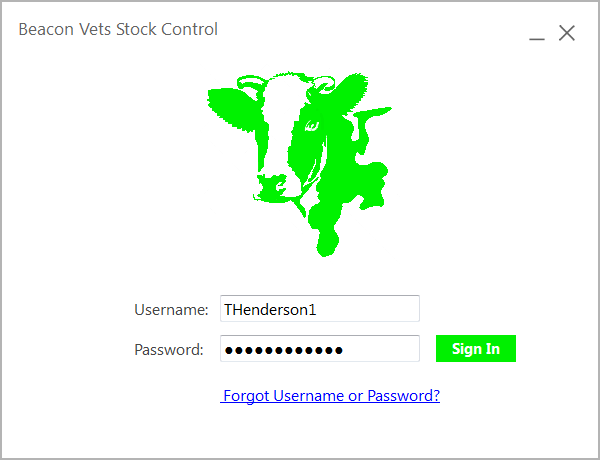
\includegraphics[width=\textwidth]{./101-1.png}
    \caption{Entering Valid Log In Details At The Log In Screen} \label{fig:101-1}
\end{figure}

\begin{figure}[H]
    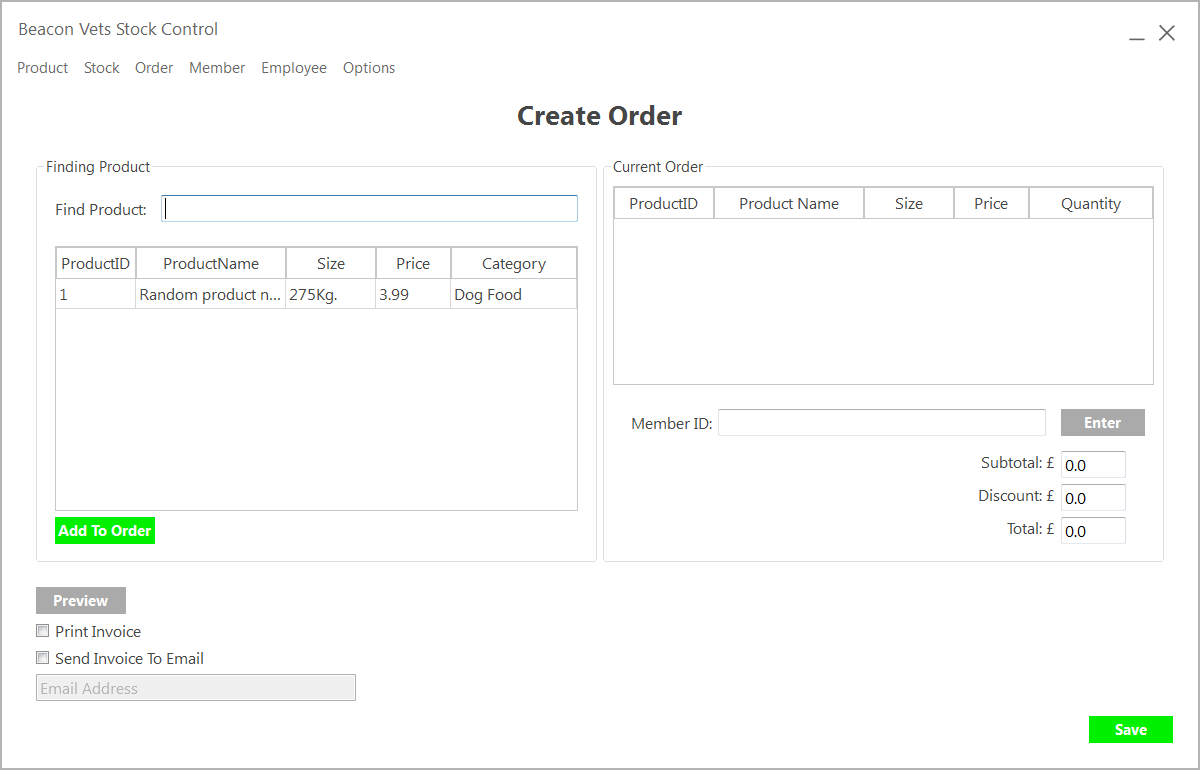
\includegraphics[width=\textwidth]{./101-2.png}
    \caption{Clicking Log In Button with Valid Details} \label{fig:101-2}
\end{figure}

\begin{figure}[H]
    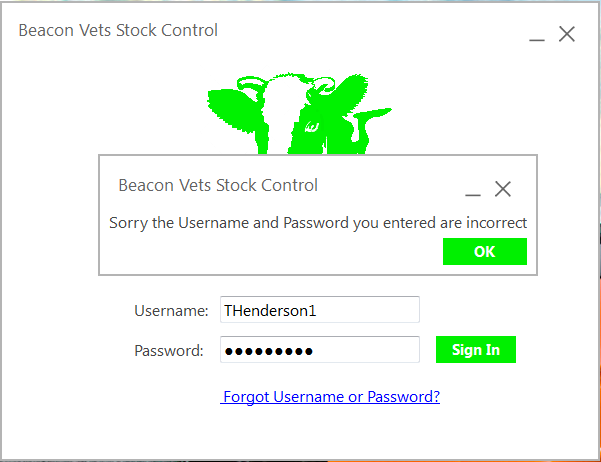
\includegraphics[width=\textwidth]{./101-3.png}
    \caption{Trying to sign in with invalid details} \label{fig:101-3}
\end{figure}

\begin{figure}[H]
    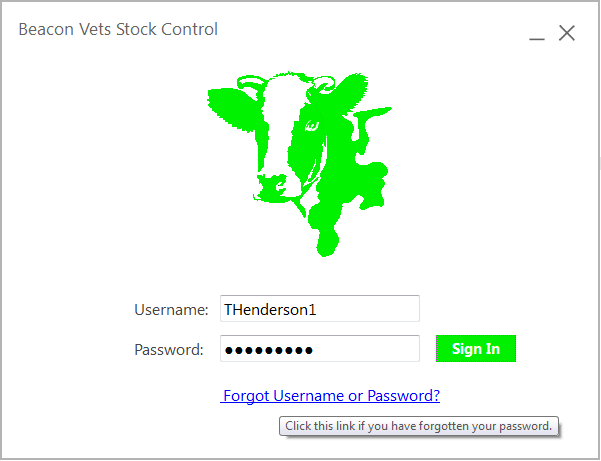
\includegraphics[width=\textwidth]{./102-1.png}
    \caption{Clicking Forgot Username or Password Button} \label{fig:102-1}
\end{figure}

\begin{figure}[H]
    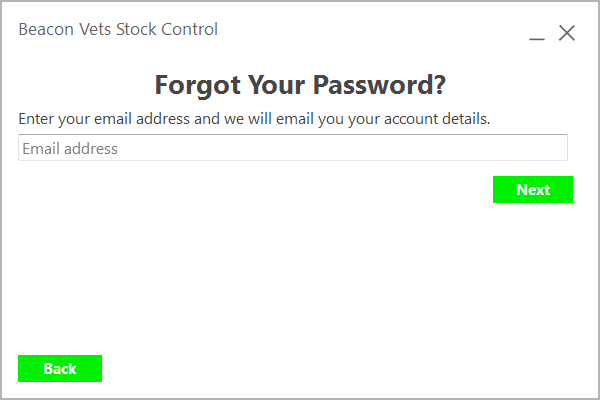
\includegraphics[width=\textwidth]{./102-2.png}
    \caption{After Clicking on the Forgot Password Button } \label{fig:102-2}
\end{figure}

\begin{figure}[H]
    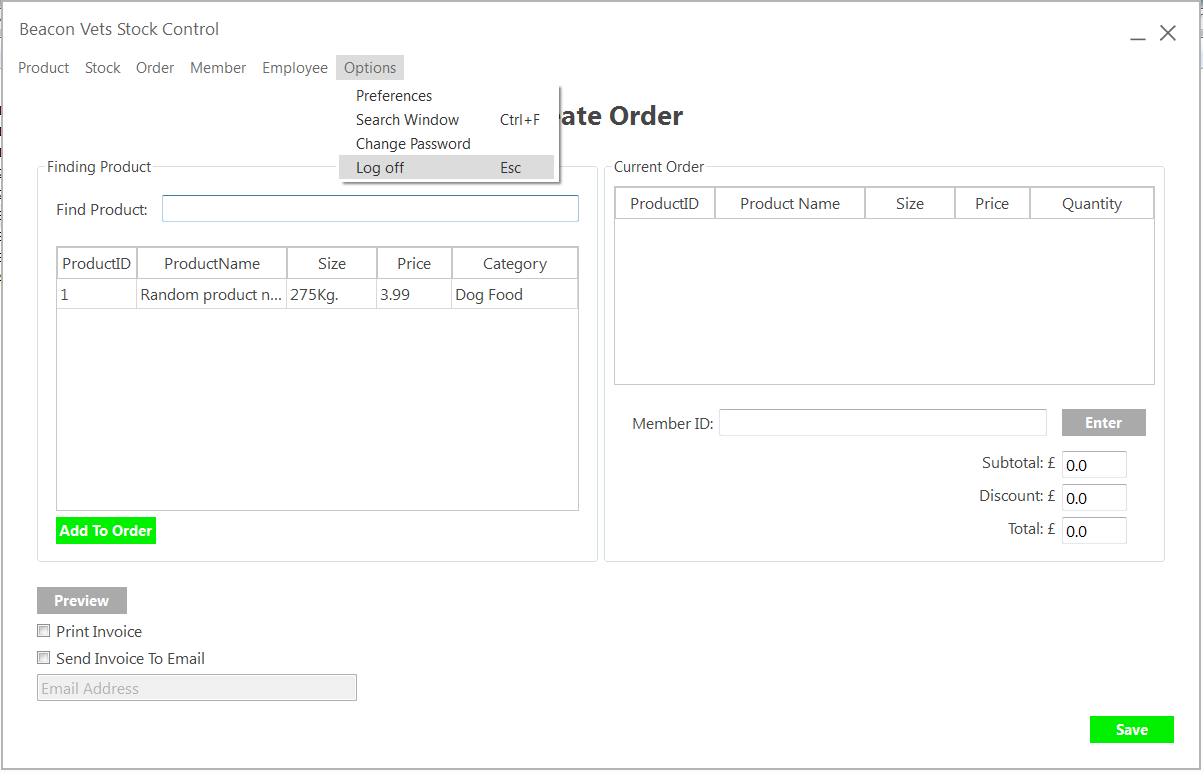
\includegraphics[width=\textwidth]{./103-1.png}
    \caption{Clicking The Log Off button} \label{fig:103-1}
\end{figure}

\begin{figure}[H]
    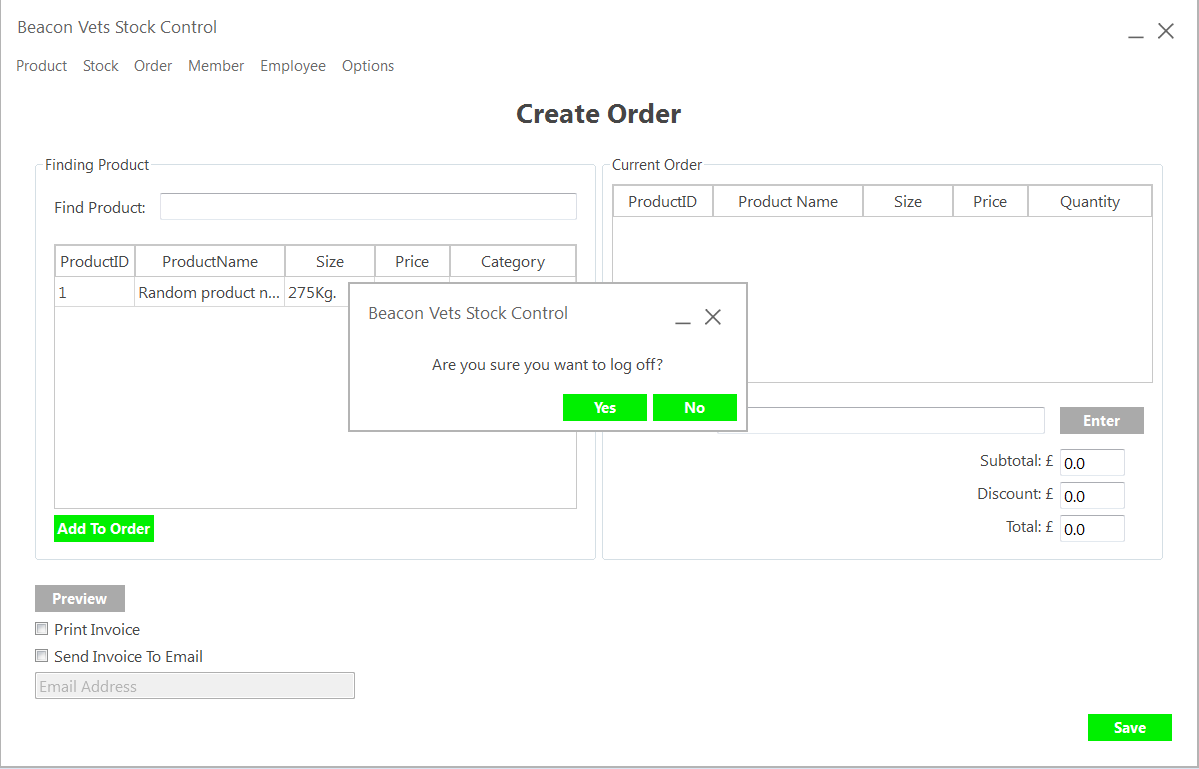
\includegraphics[width=\textwidth]{./103-2.png}
    \caption{Log Off Confirmation Window} \label{fig:103-2}
\end{figure}

\begin{figure}[H]
    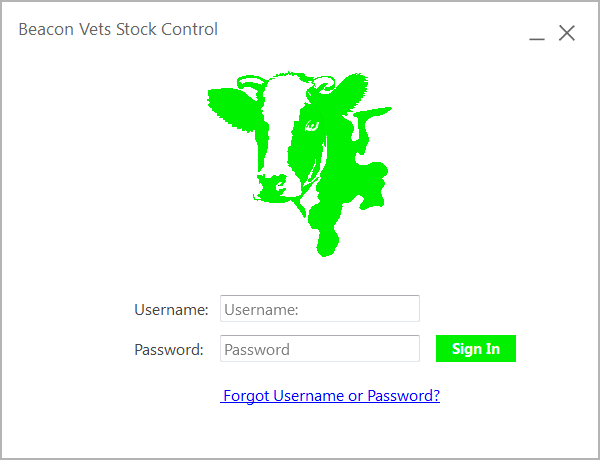
\includegraphics[width=\textwidth]{./103-3.png}
    \caption{After Clicking Yes on the Log Off Decision} \label{fig:103-3}
\end{figure}

\begin{figure}[H]
    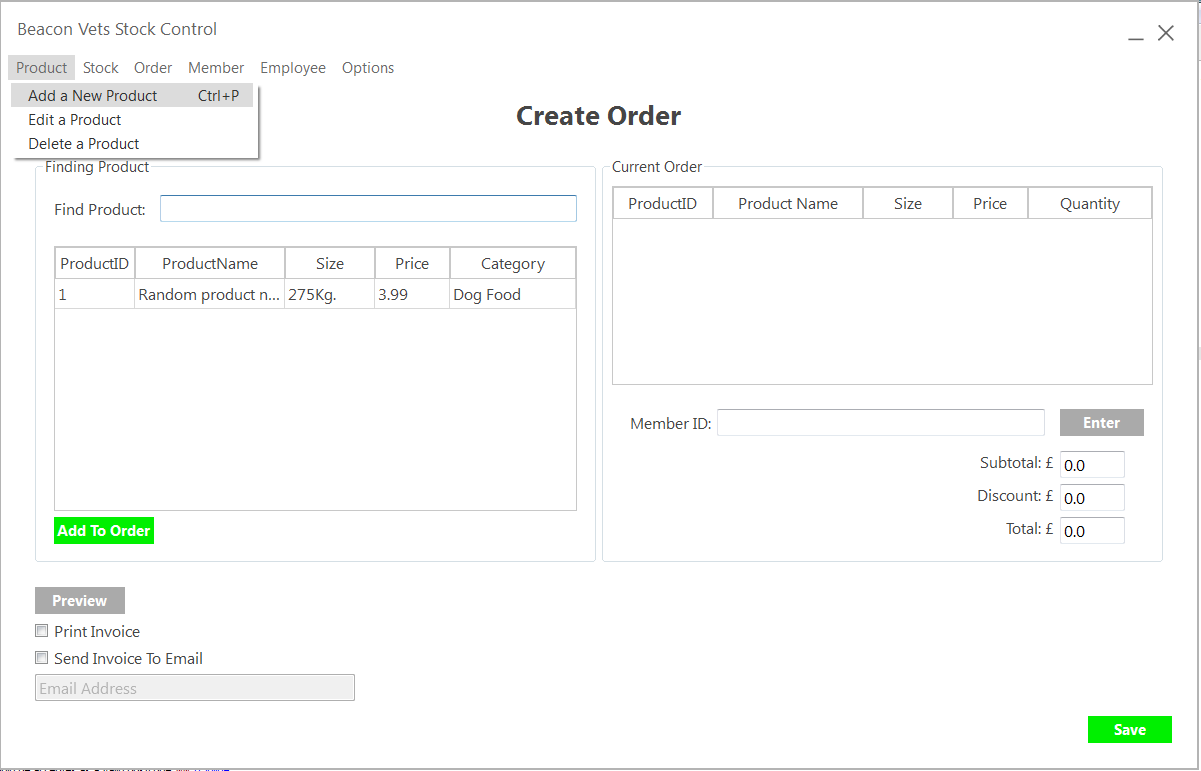
\includegraphics[width=\textwidth]{./104-1.png}
    \caption{Clicking The Add Product Button Under The Product Menu} \label{fig:104-1}
\end{figure}

\begin{figure}[H]
    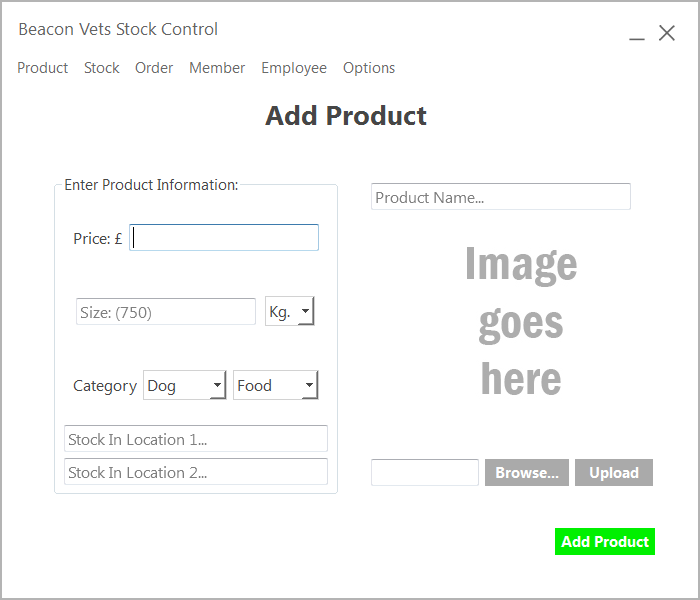
\includegraphics[width=\textwidth]{./104-2.png}
    \caption{The Add Product Interface} \label{fig:104-2}
\end{figure}

\begin{figure}[H]
    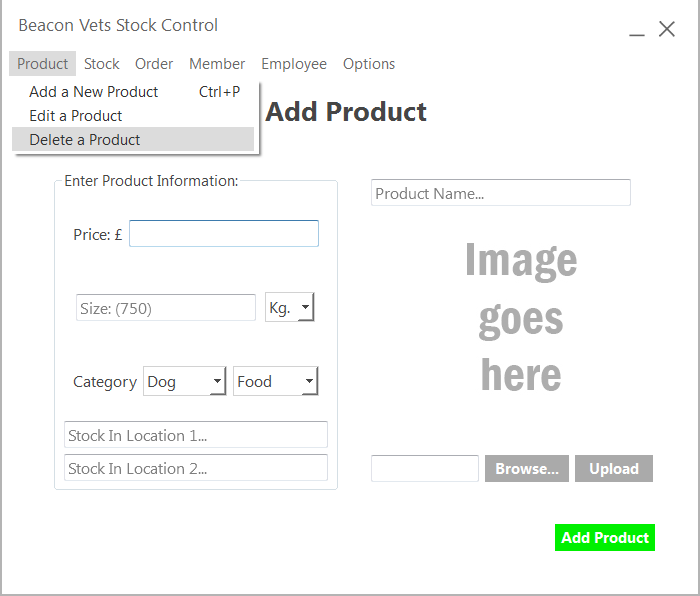
\includegraphics[width=\textwidth]{./105-1.png}
    \caption{Clicking the Delete Product Button Under the Product Menu} \label{fig:105-1}
\end{figure}

\begin{figure}[H]
    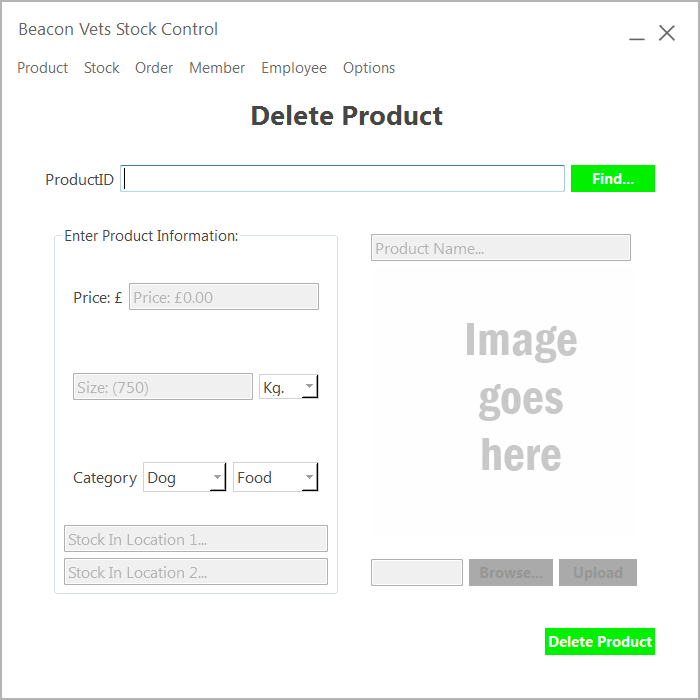
\includegraphics[width=\textwidth]{./105-2.png}
    \caption{Delete Product Interface} \label{fig:105-2}
\end{figure}

\begin{figure}[H]
    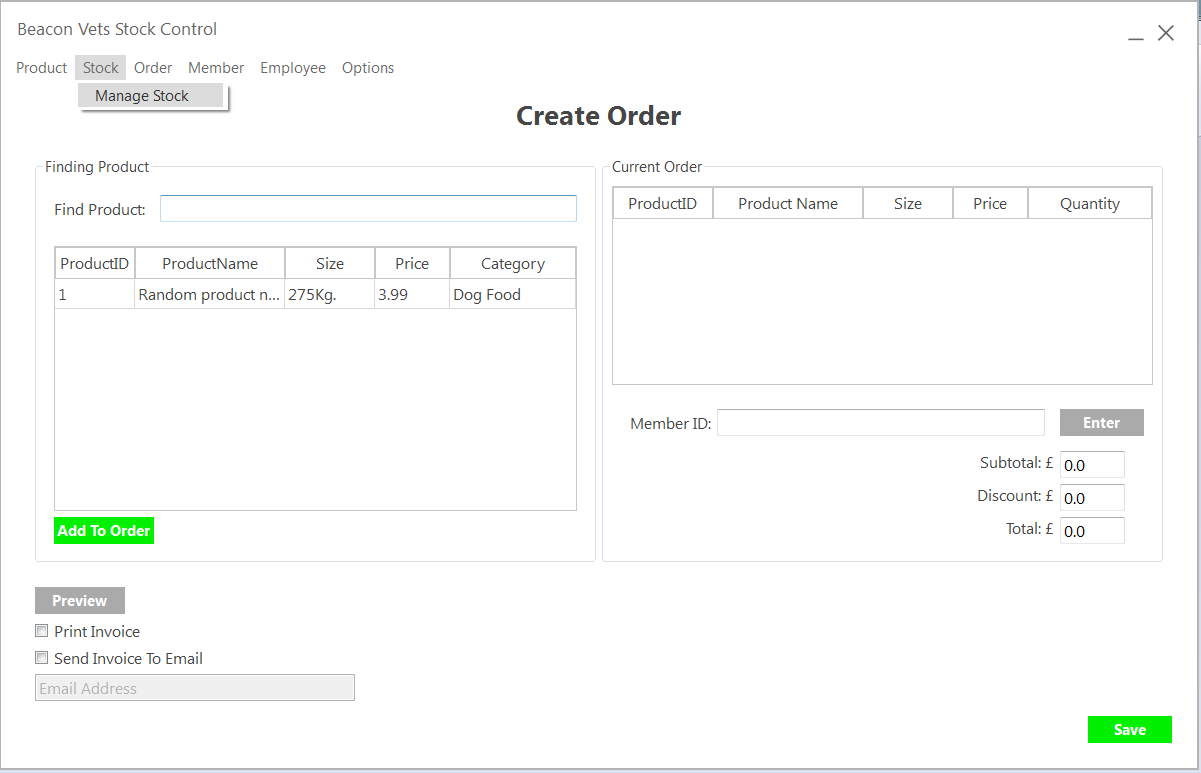
\includegraphics[width=\textwidth]{./106-1.png}
    \caption{Clicking the Manage Stock Button Under the Stock Menu.} \label{fig:106-1}
\end{figure}

\begin{figure}[H]
    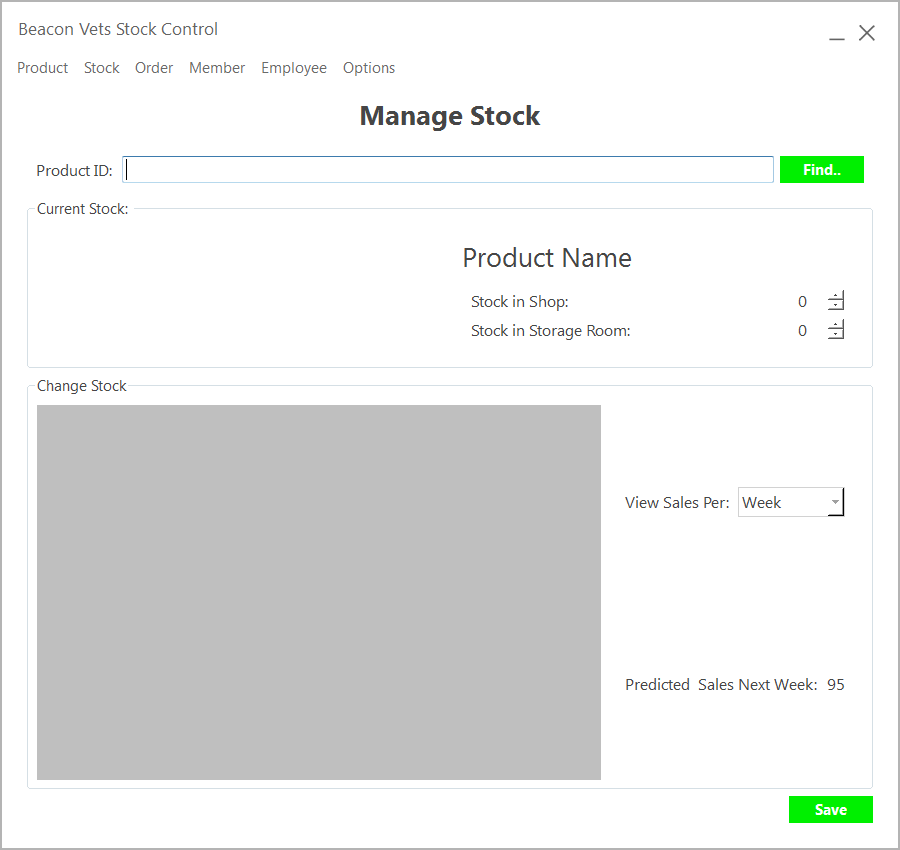
\includegraphics[width=\textwidth]{./106-2.png}
    \caption{Manage Stock Interface} \label{fig:106-2}
\end{figure}

\begin{figure}[H]
    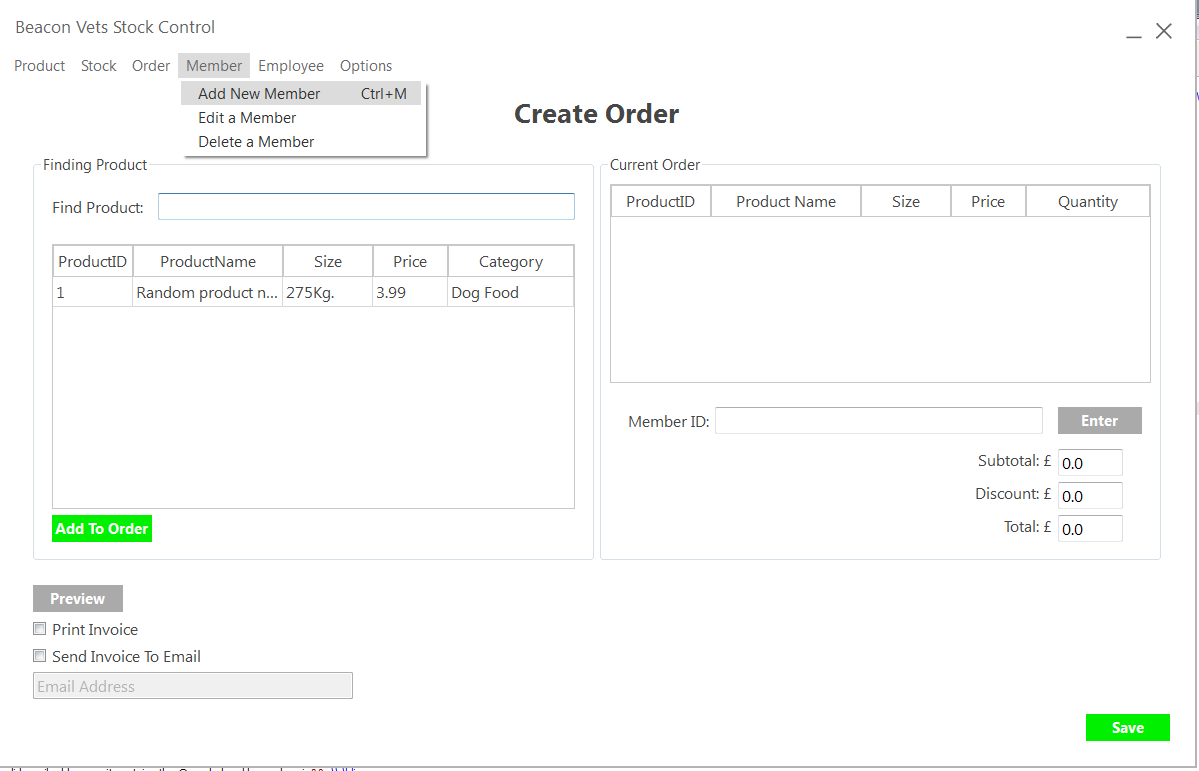
\includegraphics[width=\textwidth]{./107-1.png}
    \caption{Clicking the Adding Member Interface} \label{fig:107-1}
\end{figure}

\begin{figure}[H]
    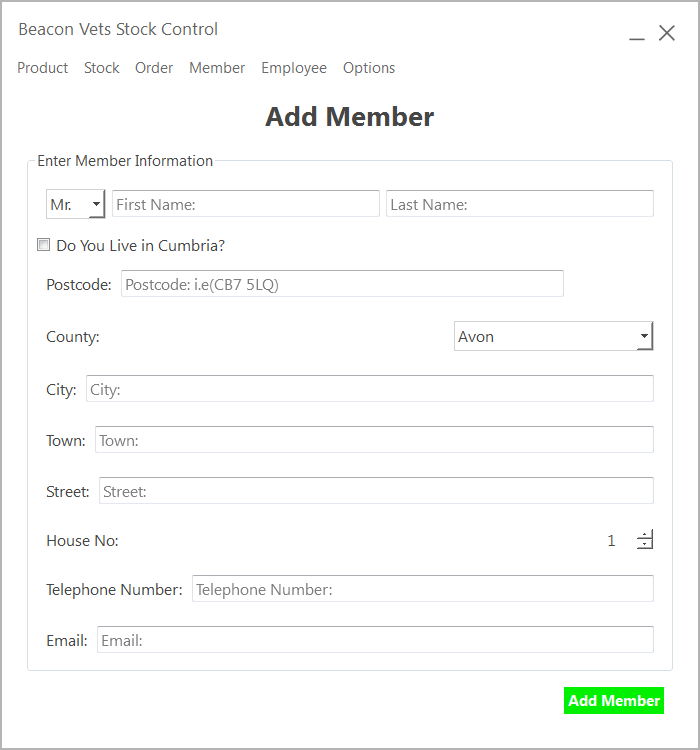
\includegraphics[width=\textwidth]{./107-2.png}
    \caption{Adding Member Interface} \label{fig:107-2}
\end{figure}

\begin{figure}[H]
    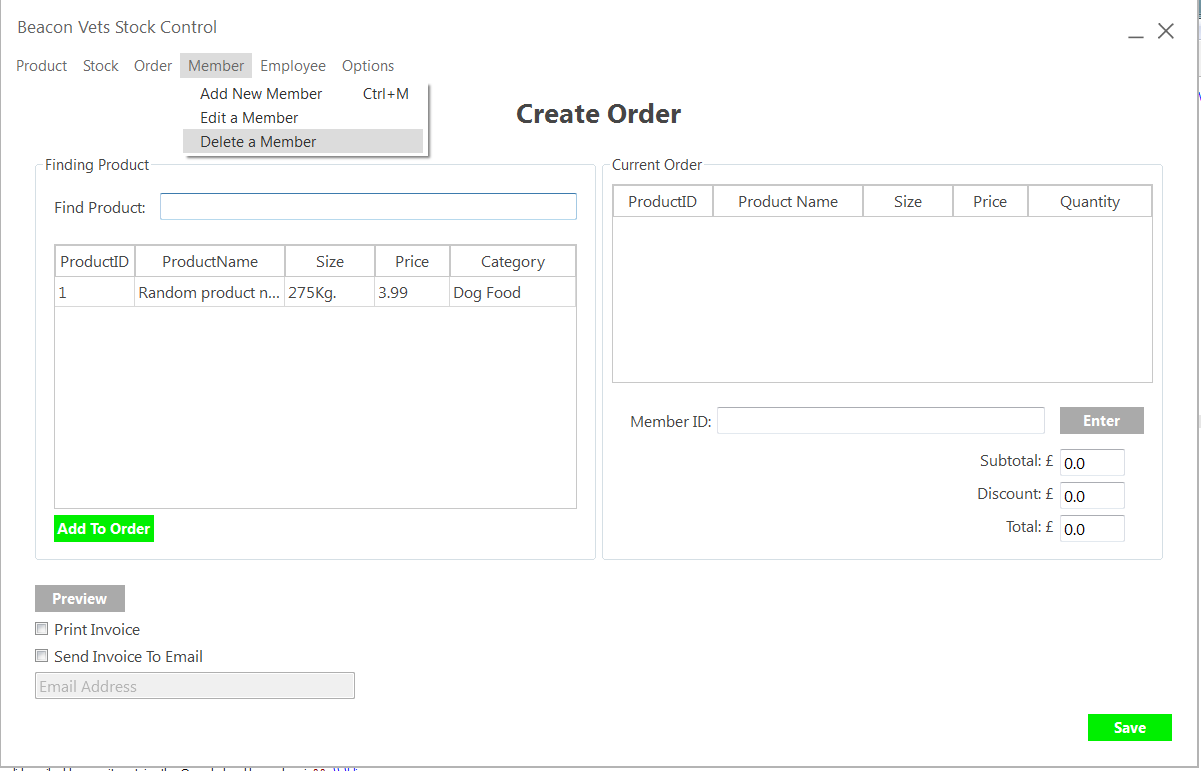
\includegraphics[width=\textwidth]{./108-1.png}
    \caption{Clicking the Delete Member Option Under the Member Menu} \label{fig:108-1}
\end{figure}

\begin{figure}[H]
    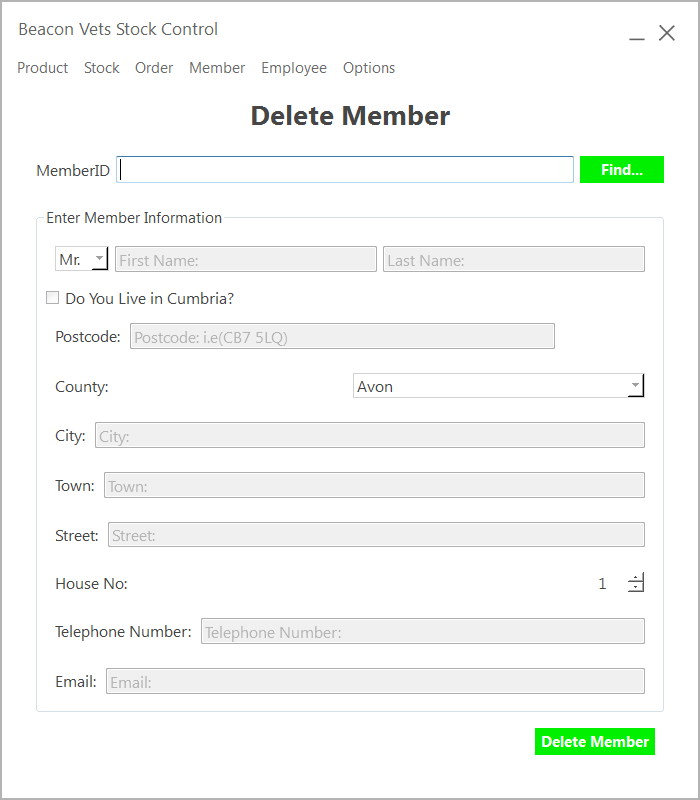
\includegraphics[width=\textwidth]{./108-2.png}
    \caption{The Delete Member Interface} \label{fig:108-2}
\end{figure}

\begin{figure}[H]
    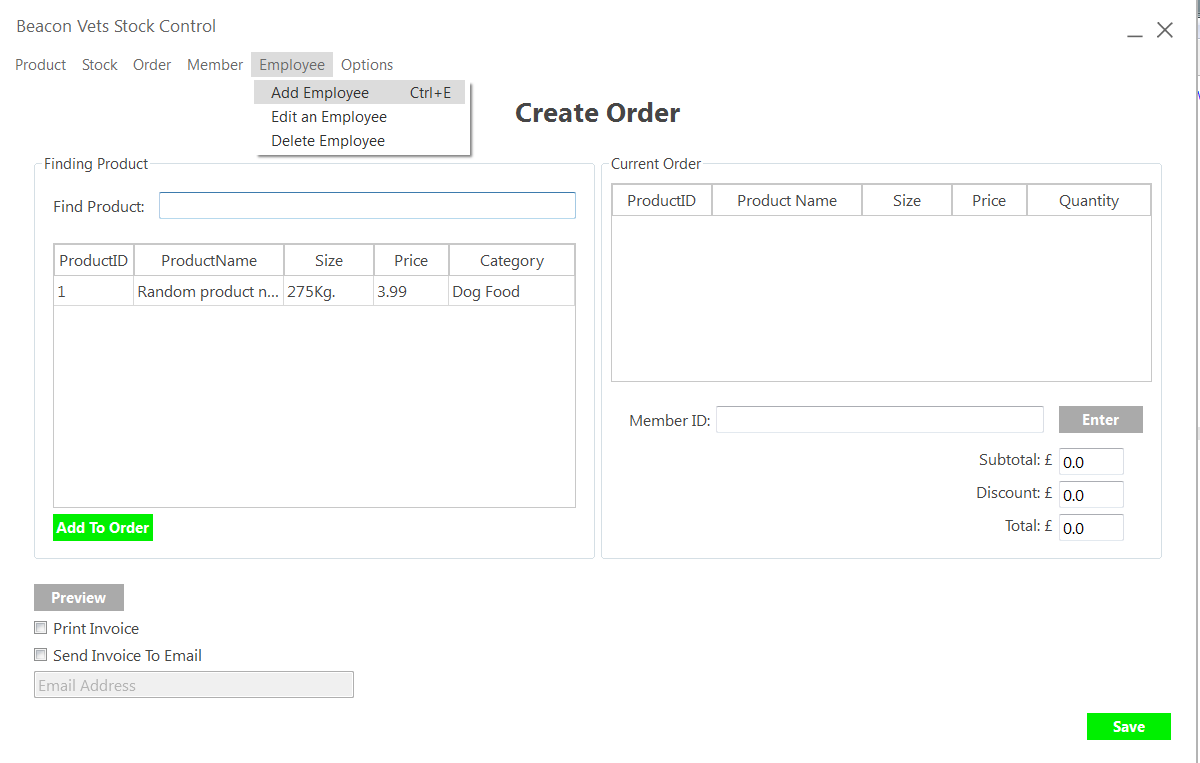
\includegraphics[width=\textwidth]{./109-1.png}
    \caption{Clicking Add Employee Button under Employee Menu} \label{fig:109-1}
\end{figure}

\begin{figure}[H]
    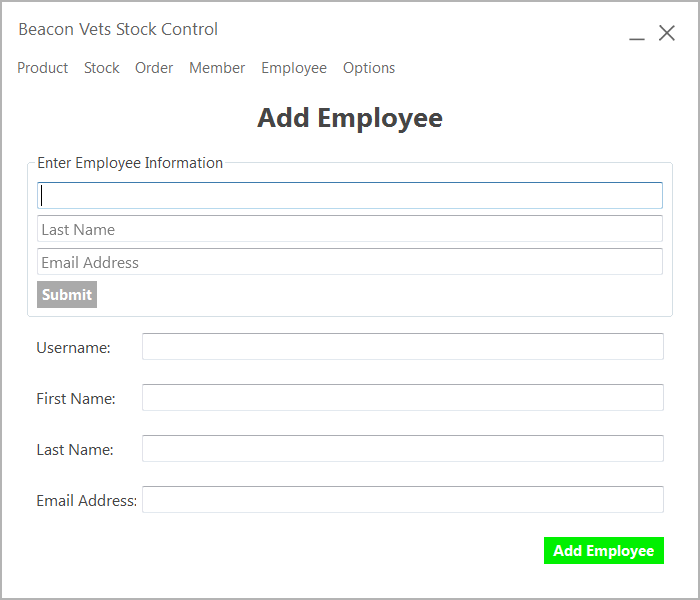
\includegraphics[width=\textwidth]{./109-2.png}
    \caption{The Add Employee Interface} \label{fig:109-2}
\end{figure}

\begin{figure}[H]
    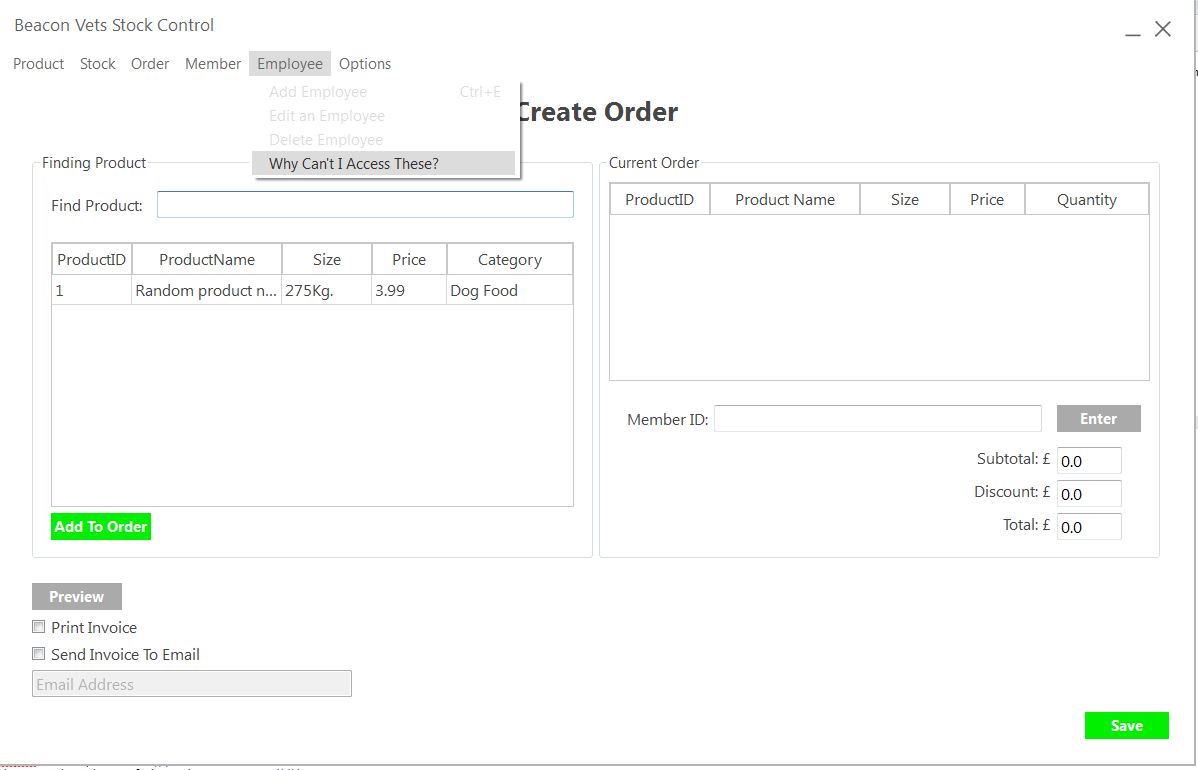
\includegraphics[width=\textwidth]{./109-3.png}
    \caption{Menu that is displayed When not Logged in on the Administrator Account} \label{fig:109-3}
\end{figure}

\begin{figure}[H]
    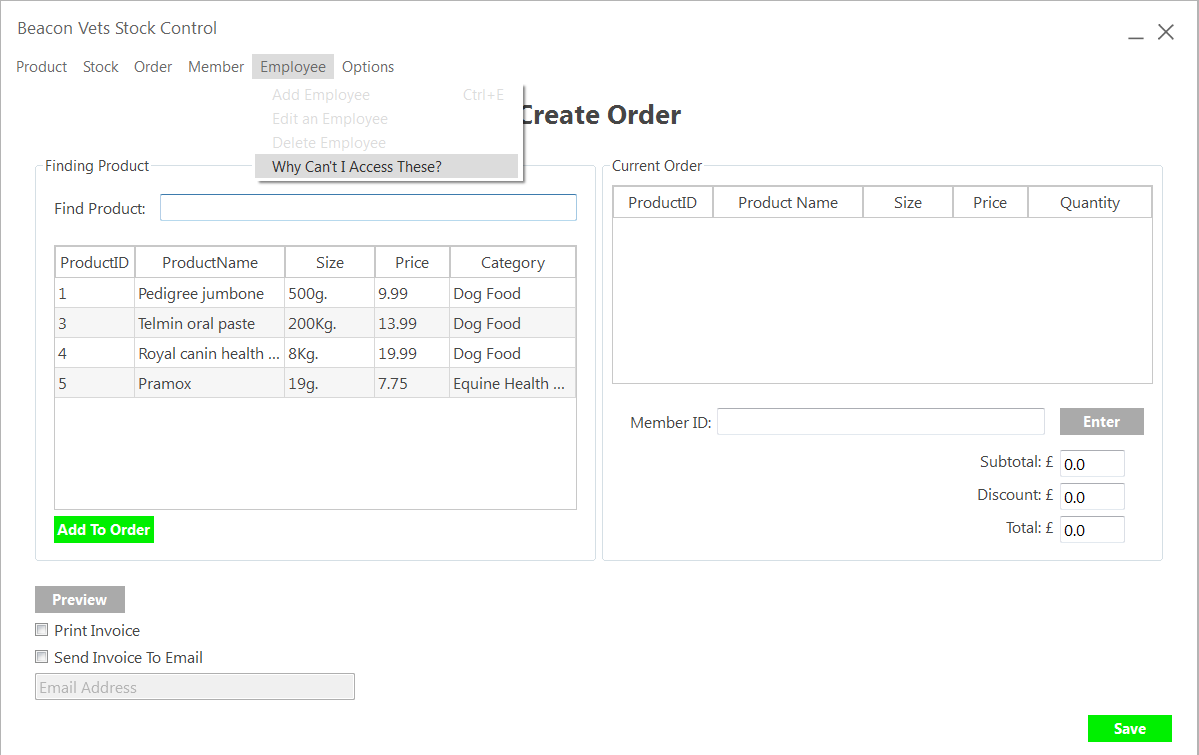
\includegraphics[width=\textwidth]{./110-1.png}
    \caption{Clicking on the why can't i access this option under the Employee menu, if the user is not signed in on the administrators account.} \label{fig:110-1}
\end{figure}

\begin{figure}[H]
    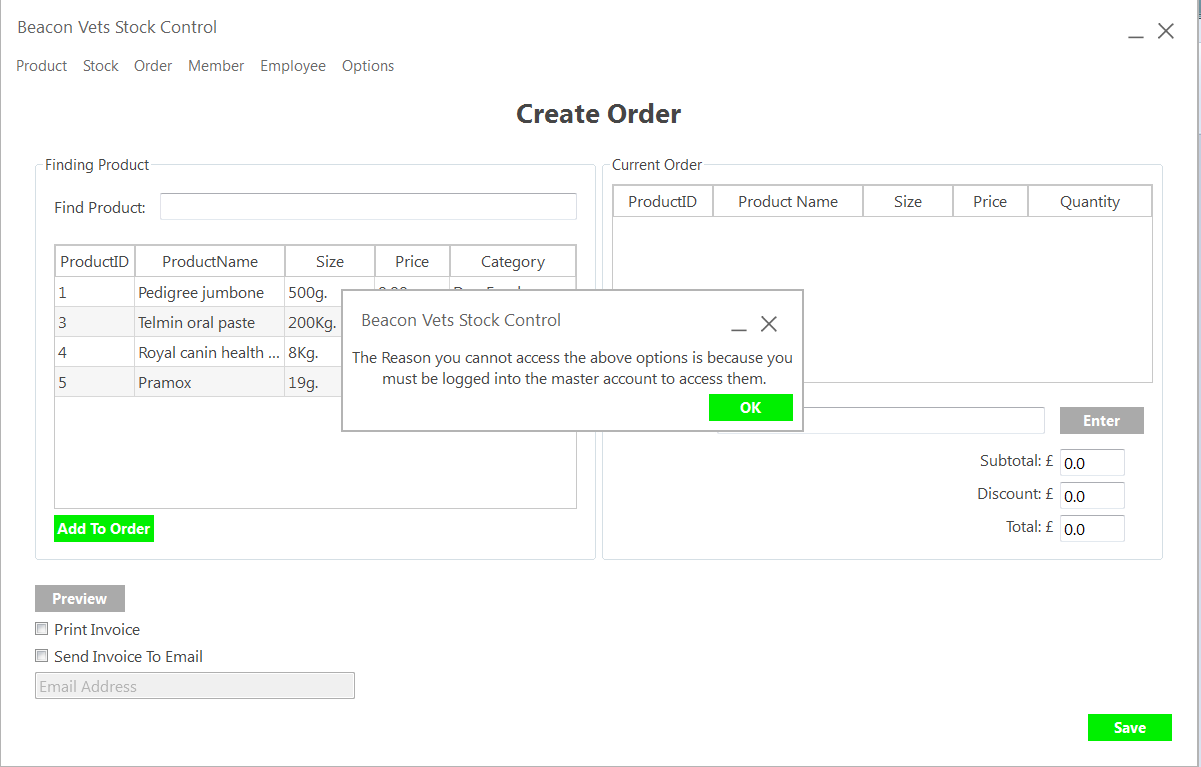
\includegraphics[width=\textwidth]{./110-2.png}
    \caption{A message being displayed when they click on the `Why can't i access this' option under the employee menu.} \label{fig:110-2}
\end{figure}

\begin{figure}[H]
    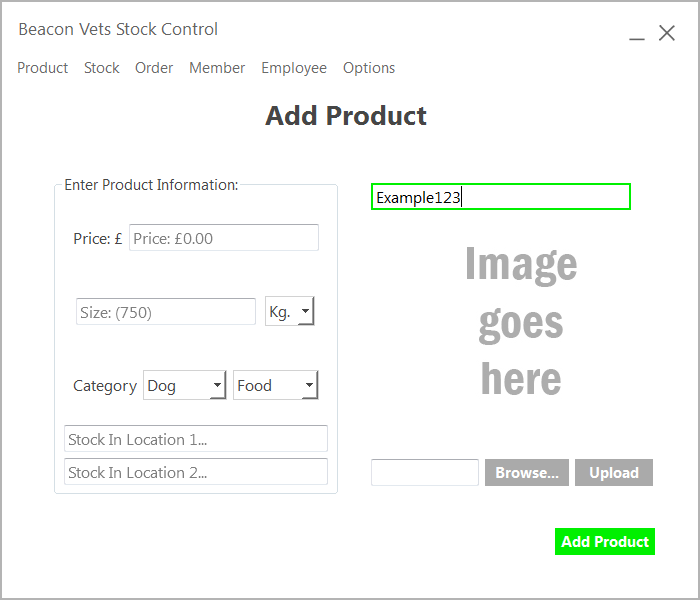
\includegraphics[width=\textwidth]{./201-1.png}
    \caption{Entering a Test into the Product Name field.} \label{fig:201-1}
\end{figure}

\begin{figure}[H]
    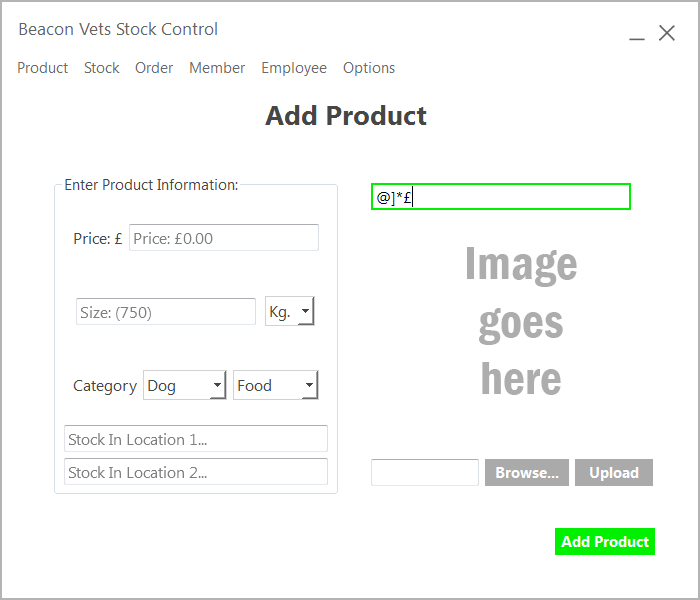
\includegraphics[width=\textwidth]{./201-2.png}
    \caption{Entering Special Characters into the Product Name field.} \label{fig:201-2}
\end{figure}

\begin{figure}[H]
    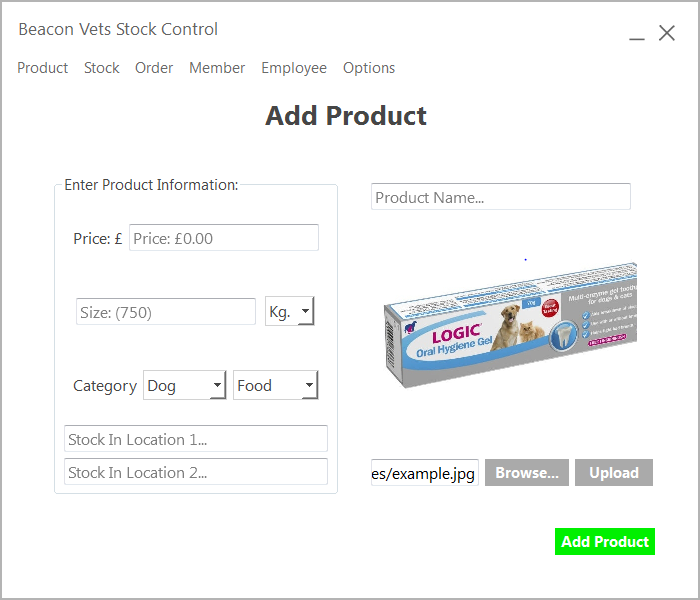
\includegraphics[width=\textwidth]{./202-1.png}
    \caption{using the exmaple.jpg image, and The Image being displayed in the image box.} \label{fig:202-1}
\end{figure}

\begin{figure}[H]
    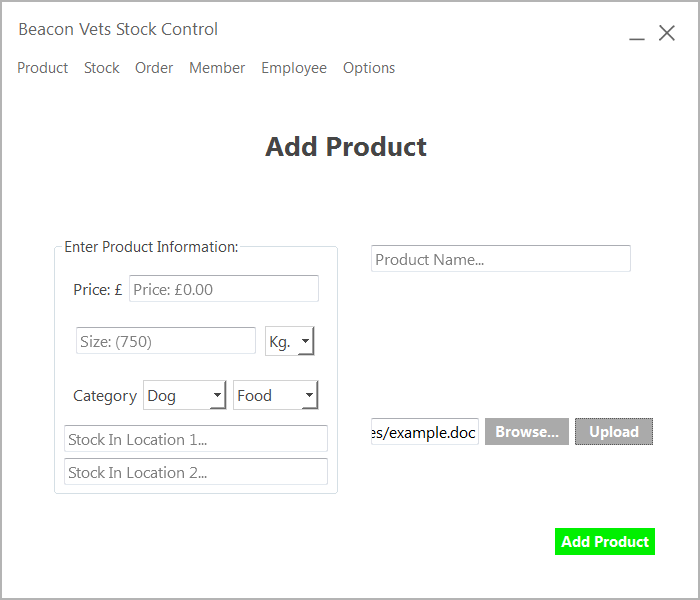
\includegraphics[width=\textwidth]{./202-2.png}
    \caption{Changing the path to an invalid image type.} \label{fig:202-2}
\end{figure}

\begin{figure}[H]
    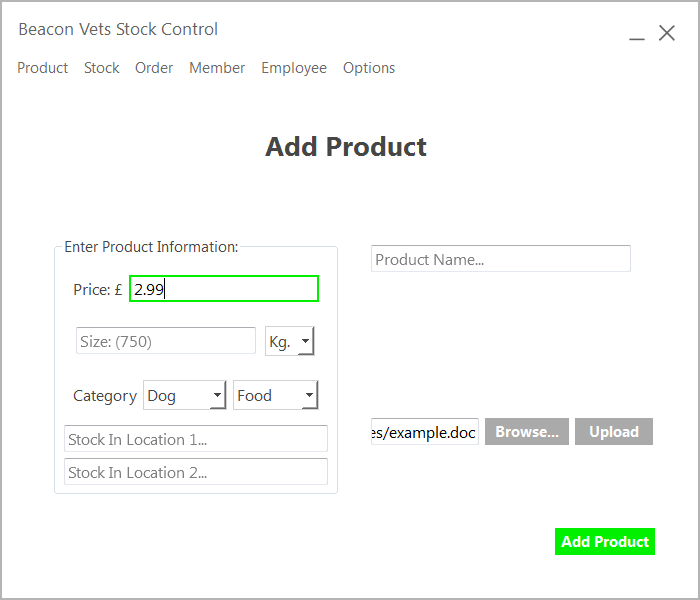
\includegraphics[width=\textwidth]{./203-1.png}
    \caption{Entering Test data into the Price field.} \label{fig:203-1}
\end{figure}

\begin{figure}[H]
    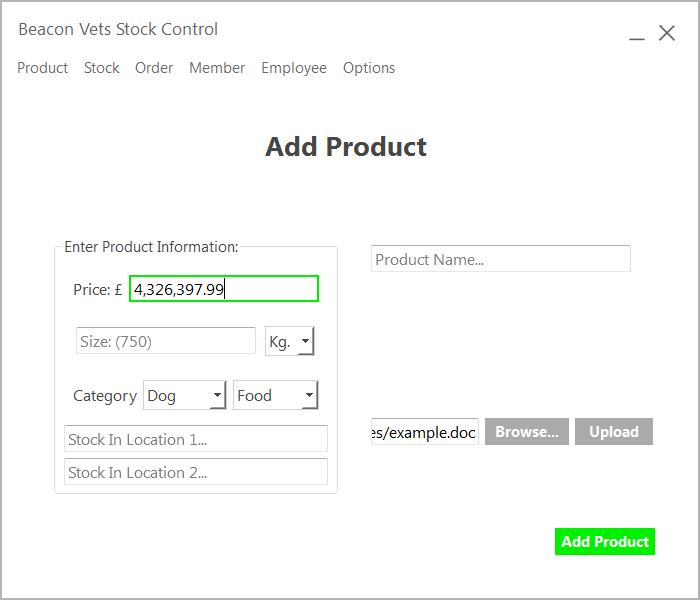
\includegraphics[width=\textwidth]{./203-2.png}
    \caption{Testing the Boundaries of the Price field.} \label{fig:203-2}
\end{figure}

\begin{figure}[H]
    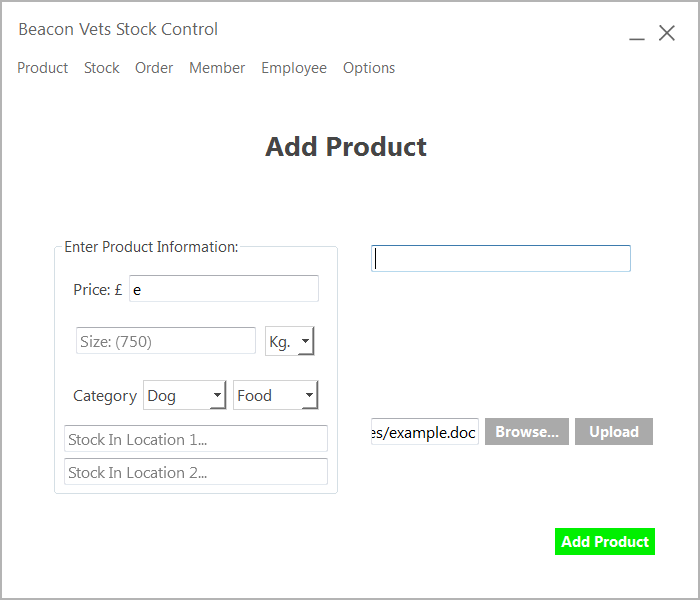
\includegraphics[width=\textwidth]{./203-3.png}
    \caption{Entering example into the price field} \label{fig:203-3}
\end{figure}

\begin{figure}[H]
    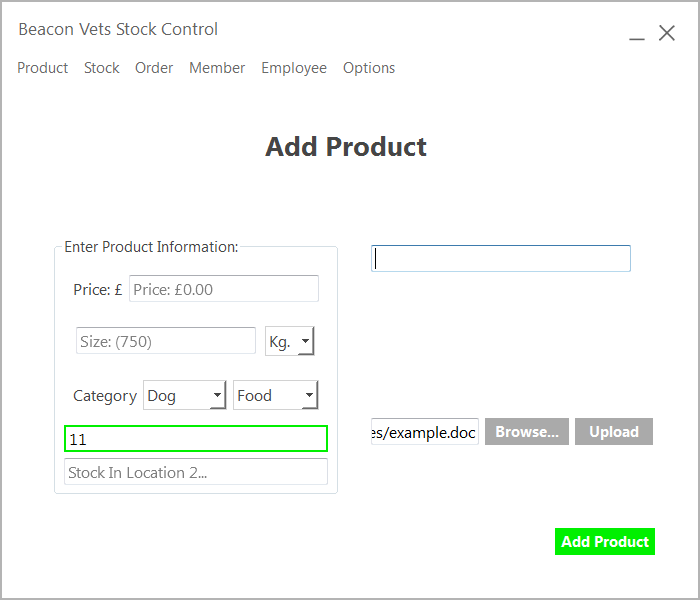
\includegraphics[width=\textwidth]{./204-1.png}
    \caption{Entering Test data into the stock field.} \label{fig:204-1}
\end{figure}

\begin{figure}[H]
    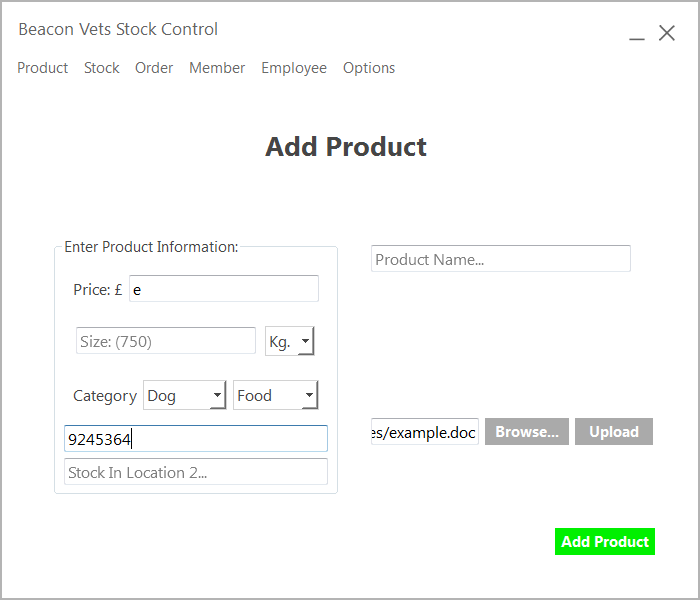
\includegraphics[width=\textwidth]{./204-2.png}
    \caption{Testing the boundaries of the Stock field} \label{fig:204-2}
\end{figure}

\begin{figure}[H]
    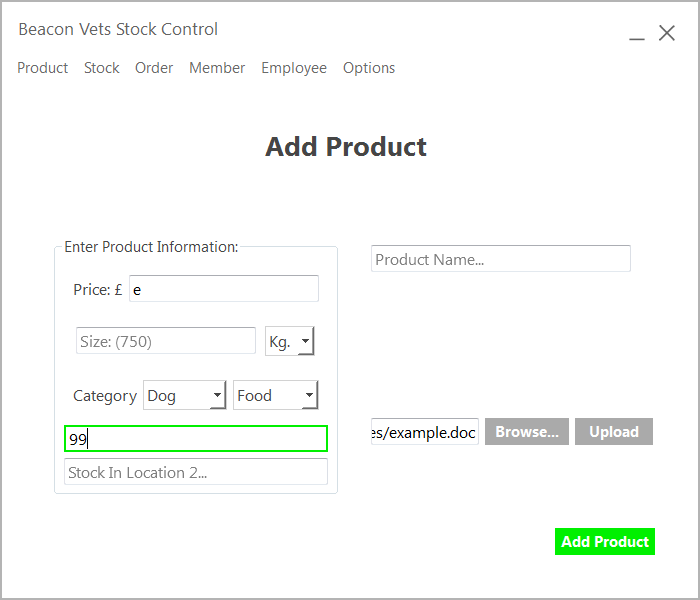
\includegraphics[width=\textwidth]{./204-3.png}
    \caption{Entering 99 in the Stock field} \label{fig:204-3}
\end{figure}

\begin{figure}[H]
    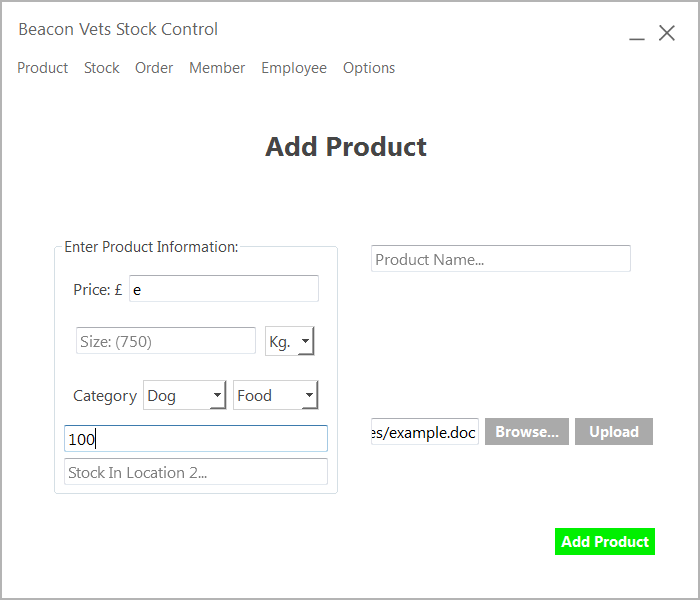
\includegraphics[width=\textwidth]{./204-4.png}
    \caption{Entering 100 into the Stock field.} \label{fig:204-4}
\end{figure}

\begin{figure}[H]
    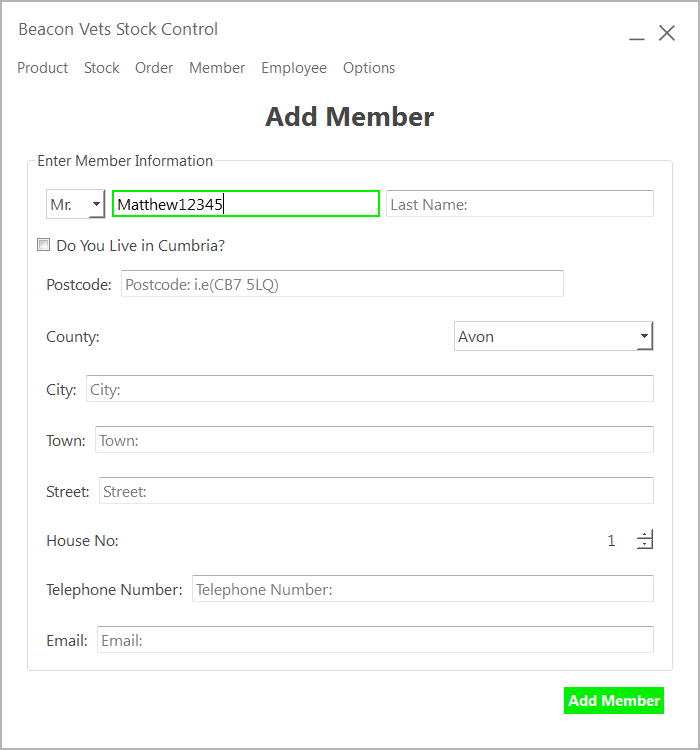
\includegraphics[width=\textwidth]{./205-1.png}
    \caption{Entering Letters and Numbers into the Member First Name field} \label{fig:205-1}
\end{figure}

\begin{figure}[H]
    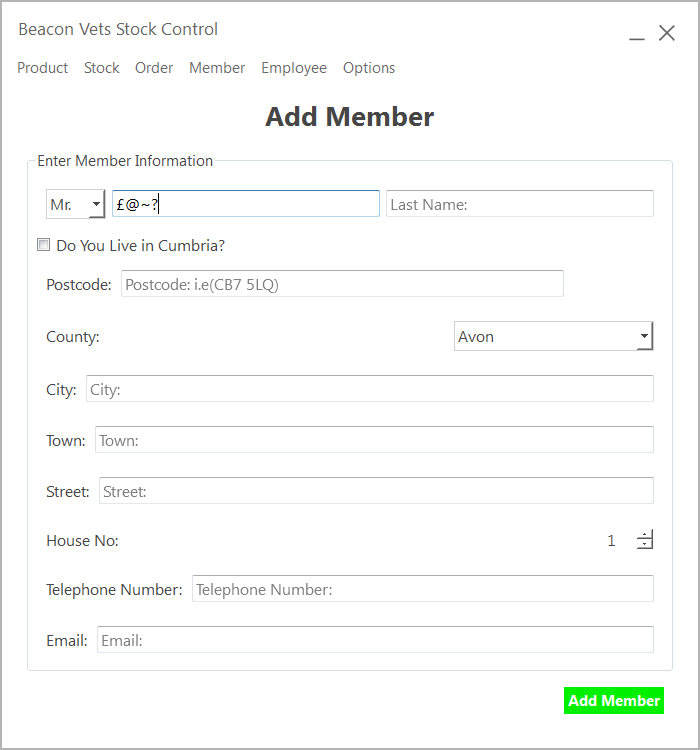
\includegraphics[width=\textwidth]{./205-2.png}
    \caption{Entering special characters into the Members first Name Field} \label{fig:205-2}
\end{figure}

\begin{figure}[H]
    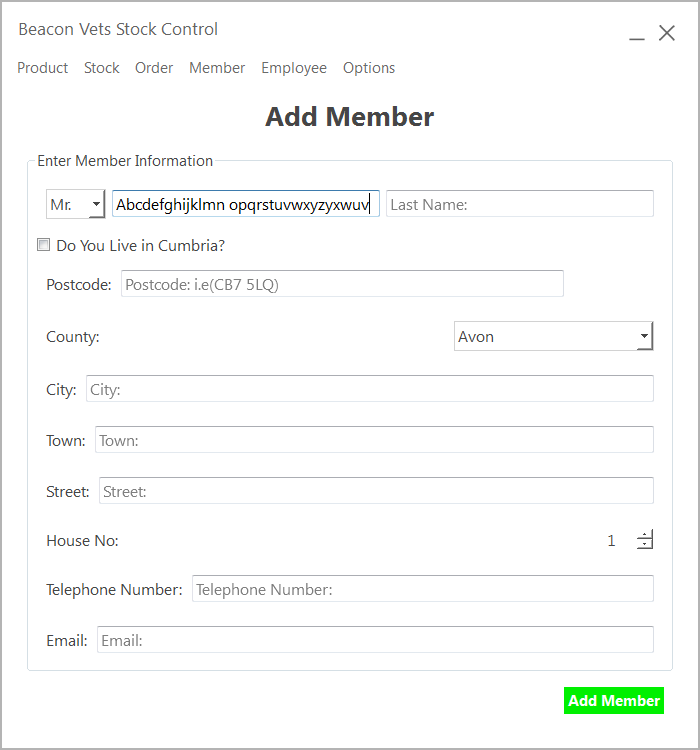
\includegraphics[width=\textwidth]{./205-3.png}
    \caption{Entering a name outside the boundary of the Member First Name} \label{fig:205-3}
\end{figure}

\begin{figure}[H]
    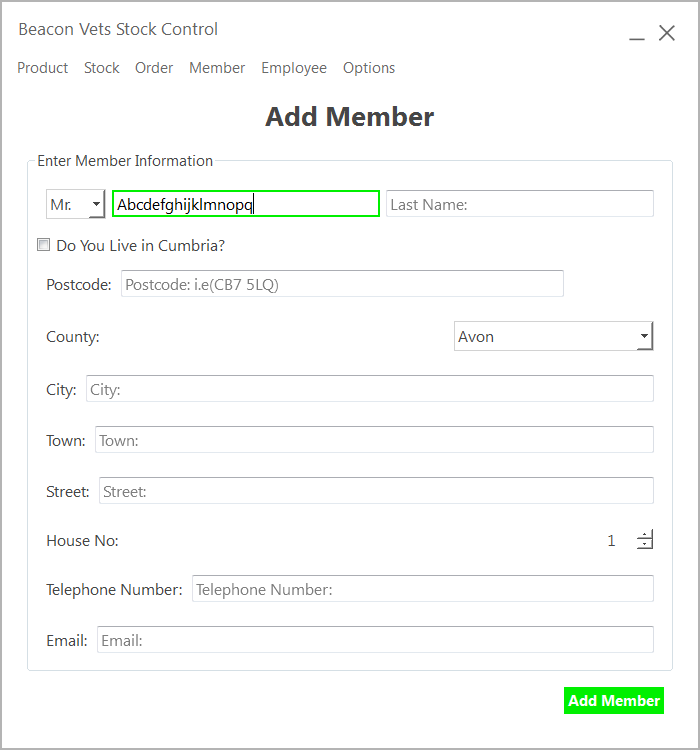
\includegraphics[width=\textwidth]{./205-4.png}
    \caption{Entering a name just inside the boundary of the Member First Name field} \label{fig:205-4}
\end{figure}

\begin{figure}[H]
    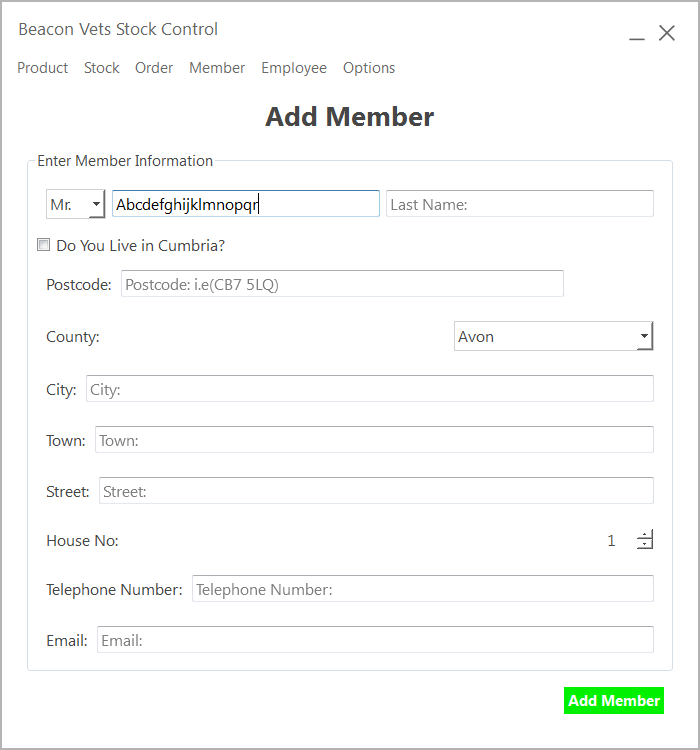
\includegraphics[width=\textwidth]{./205-5.png}
    \caption{Entering a name just outside the boundary of the Member First Name field} \label{fig:205-5}
\end{figure}

\begin{figure}[H]
    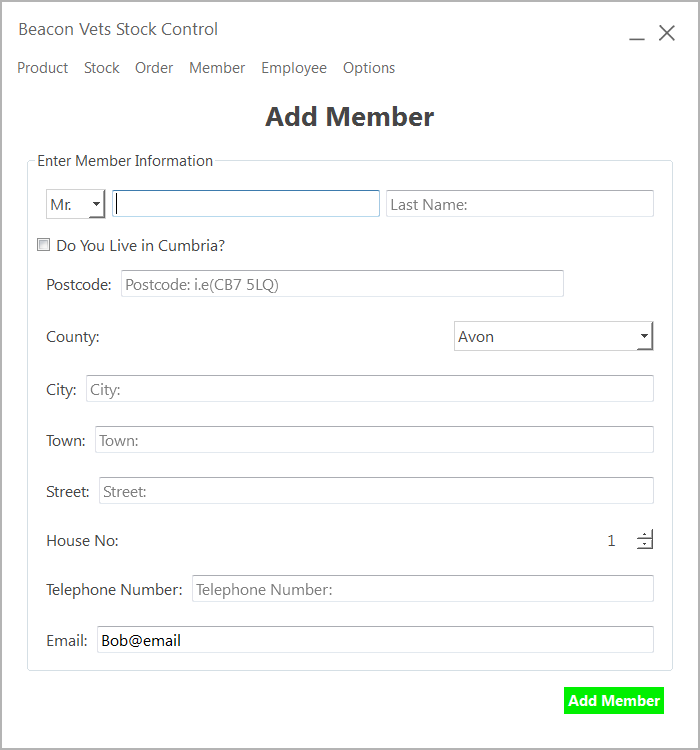
\includegraphics[width=\textwidth]{./206-1.png}
    \caption{Entering test Data into Member Email field.} \label{fig:206-1}
\end{figure}

\begin{figure}[H]
    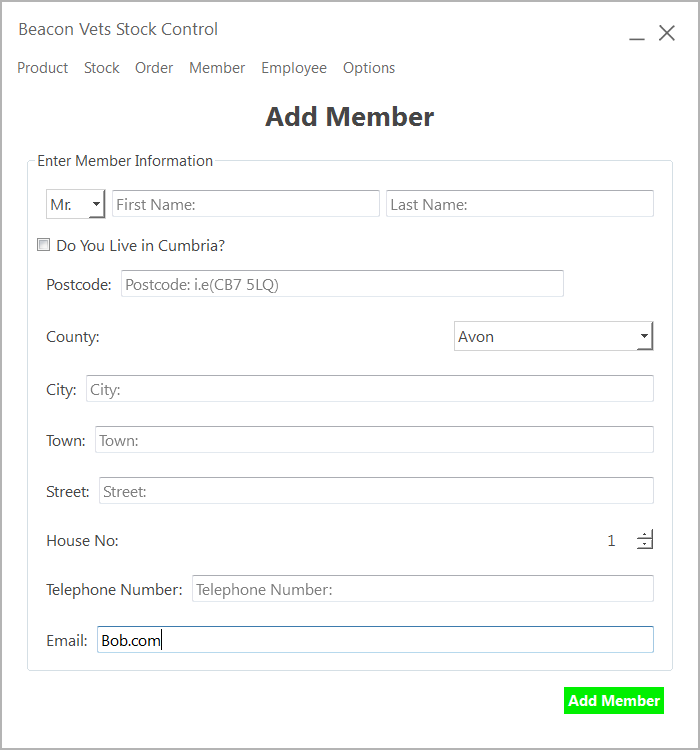
\includegraphics[width=\textwidth]{./206-2.png}
    \caption{Entering an invalid Email address into the Email field} \label{fig:206-2}
\end{figure}

\begin{figure}[H]
    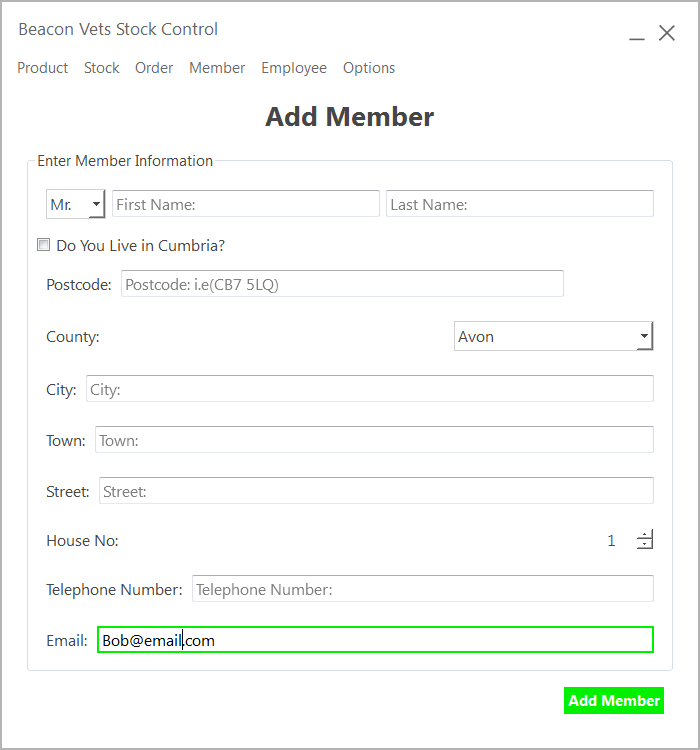
\includegraphics[width=\textwidth]{./206-3.png}
    \caption{Entering a valid Email address into the Email field} \label{fig:206-3}
\end{figure}

\begin{figure}[H]
    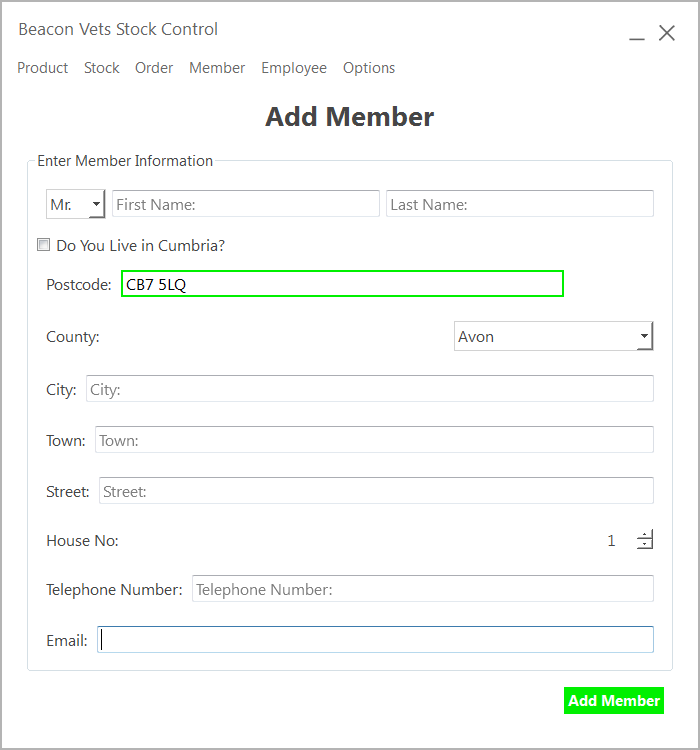
\includegraphics[width=\textwidth]{./207-1.png}
    \caption{Entering test data into the Members Postcode field.} \label{fig:207-1}
\end{figure}

\begin{figure}[H]
    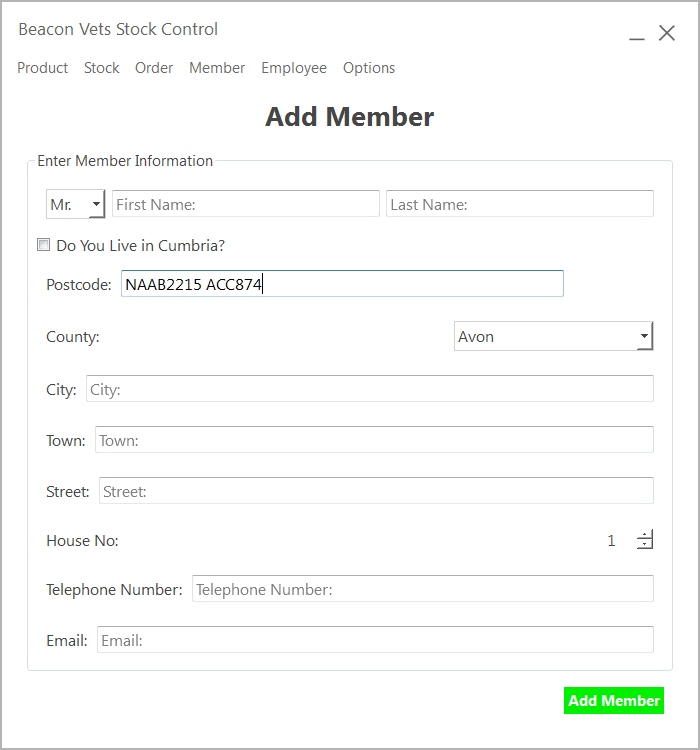
\includegraphics[width=\textwidth]{./207-2.png}
    \caption{Entering an invalid postcode into the Member Postcode field} \label{fig:207-2}
\end{figure}

\begin{figure}[H]
    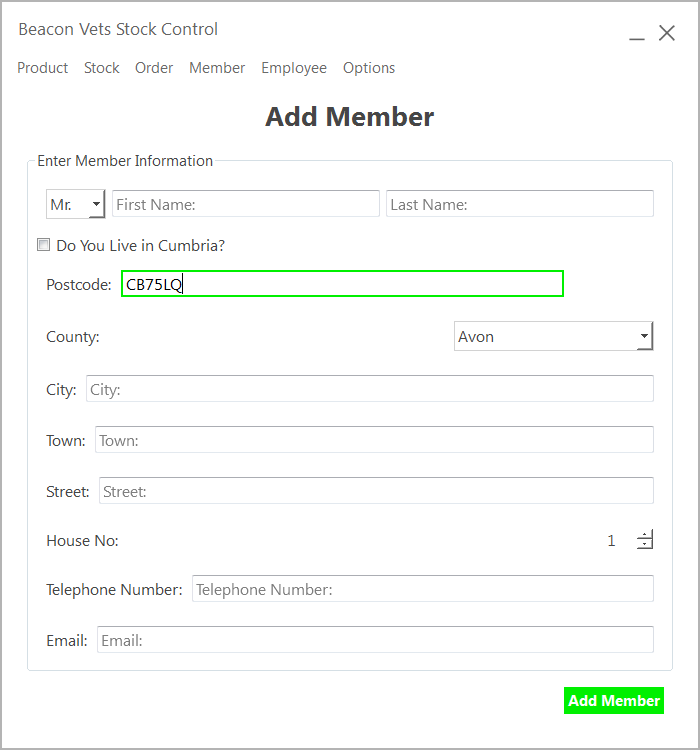
\includegraphics[width=\textwidth]{./207-3.png}
    \caption{Entering a legitimate postcode into the Postcode field} \label{fig:207-3}
\end{figure}

\begin{figure}[H]
    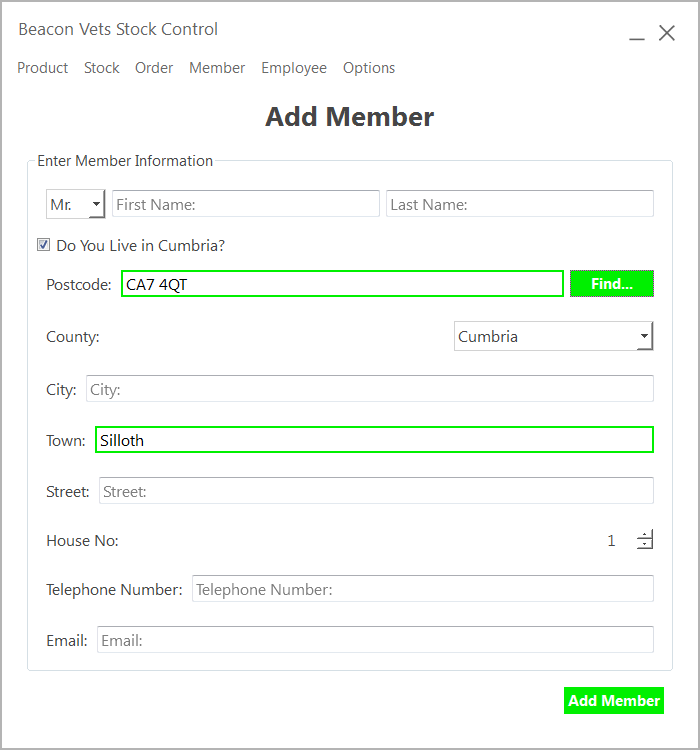
\includegraphics[width=\textwidth]{./208-1.png}
    \caption{Finding a postcode in the CSV file} \label{fig:208-1}
\end{figure}

\begin{figure}[H]
    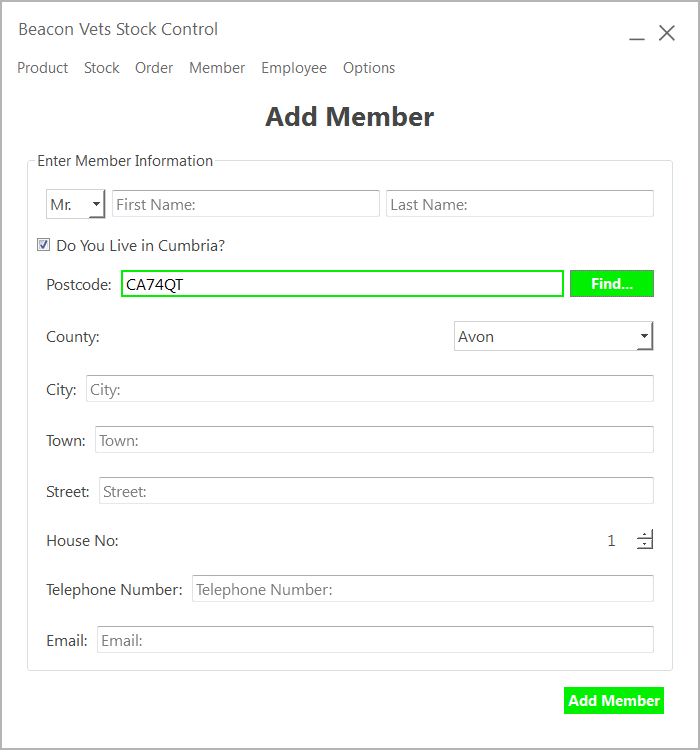
\includegraphics[width=\textwidth]{./208-2.png}
    \caption{Entering Postcode without space and not being found in the CSV file} \label{fig:208-2}
\end{figure}

\begin{figure}[H]
    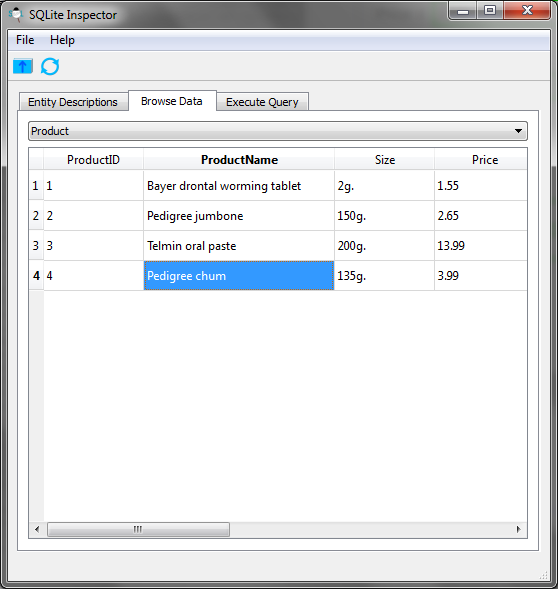
\includegraphics[width=\textwidth]{./301-1.png}
    \caption{The Product Pedigree chum being stored in the Product Name column within the Product Table.} \label{fig:301-1}
\end{figure}

\begin{figure}[H]
    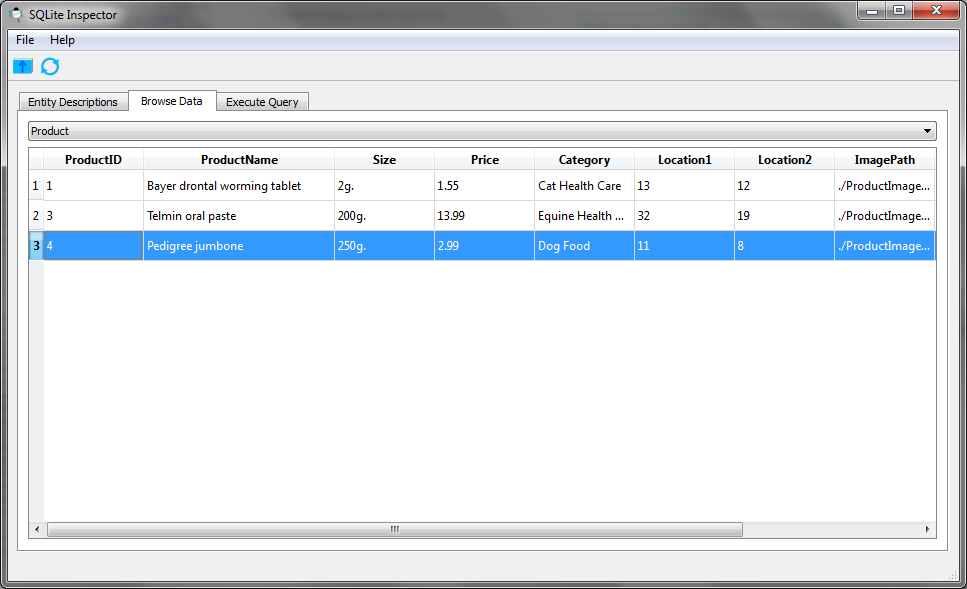
\includegraphics[width=\textwidth]{./303-1.png}
    \caption{All the Product information has been stored in the correct column within the Product table.} \label{fig:303-1}
\end{figure}

\begin{figure}[H]
    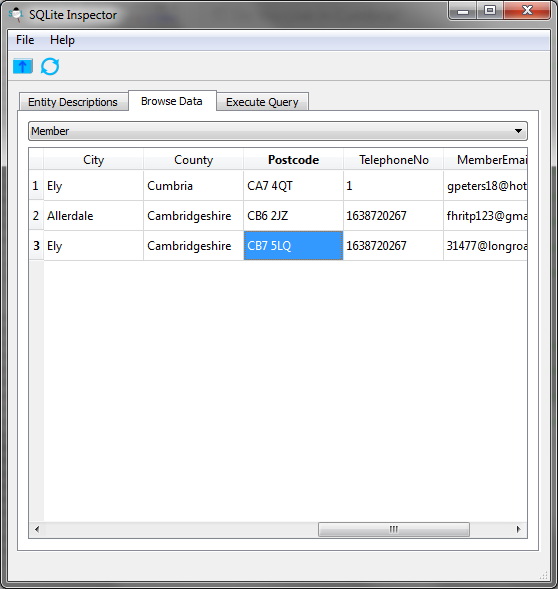
\includegraphics[width=\textwidth]{./304-1.png}
    \caption{The Postcode is stored in the correct column in the Member Table, however, the space ahs not been removed between the two parts of the postcode.} \label{fig:304-1}
\end{figure}

\begin{figure}[H]
    \includegraphics[width=\textwidth]{./305-1.png}
    \caption{All the data associated with the Member has been stored under the correct Column in the Member Table.} \label{fig:305-1}
\end{figure}

\begin{figure}[H]
    \includegraphics[width=\textwidth]{./306-1.png}
    \caption{Logging into an account for the first time using the User-name and the Password: `password' } \label{fig:306-1}
\end{figure}

\begin{figure}[H]
    \includegraphics[width=\textwidth]{./306-2.png}
    \caption{If the user password is `password', they get taken to the Change Your Password interface when logging in. } \label{fig:306-2}
\end{figure}

\begin{figure}[H]
    \includegraphics[width=\textwidth]{./308-1.png}
    \caption{The Stock of the Product in Location1 is currently 20.} \label{fig:308-1}
\end{figure}

\begin{figure}[H]
    \includegraphics[width=\textwidth]{./308-2.png}
    \caption{After Editing the Product in the system, The stock of the Product has now been changed to 15.} \label{fig:308-2}
\end{figure}

\begin{figure}[H]
    \includegraphics[width=\textwidth]{./402-1.png}
    \caption{Showing the Product information before any of the Product Data is changed.} \label{fig:402-1}
\end{figure}

\begin{figure}[H]
    \includegraphics[width=\textwidth]{./402-2.png}
    \caption{Showing the Product information has successfully changed, once updating the Product information within the system} \label{fig:402-2}
\end{figure}

\begin{figure}[H]
    \includegraphics[width=\textwidth]{./403-1.png}
    \caption{Showing the Member information before any changes are made in the system.} \label{fig:403-1}
\end{figure}

\begin{figure}[H]
    \includegraphics[width=\textwidth]{./403-2.png}
    \caption{Showing the Member information has changed after being changed within the system.} \label{fig:403-2}
\end{figure}

\begin{figure}[H]
    \includegraphics[width=\textwidth]{./404-1.png}
    \caption{Showing the Employee information before it is changed in the system.} \label{fig:404-1}
\end{figure}

\begin{figure}[H]
    \includegraphics[width=\textwidth]{./404-2.png}
    \caption{Showing the Employee information has successfully changed after being changed in the system.} \label{fig:404-2}
\end{figure}

\begin{figure}[H]
    \includegraphics[width=\textwidth]{./405-1.png}
    \caption{Showing the Products in the Product table before a Product is removed in the system.} \label{fig:405-1}
\end{figure}

\begin{figure}[H]
    \includegraphics[width=\textwidth]{./405-2.png}
    \caption{Showing that the Product with ProductID of 2 has successfully been removed from the database.} \label{fig:405-2}
\end{figure}

\begin{figure}[H]
    \includegraphics[width=\textwidth]{./406-1.png}
    \caption{Showing The Members in the database before one of them is removed.} \label{fig:406-1}
\end{figure}

\begin{figure}[H]
    \includegraphics[width=\textwidth]{./406-2.png}
    \caption{Showing That the Member with MemberID of 3 has successfully been removed from the database.} \label{fig:406-2}
\end{figure}

\begin{figure}[H]
    \includegraphics[width=\textwidth]{./407-1.png}
    \caption{Showing The Employees in the database before one of them is removed.} \label{fig:407-1}
\end{figure}

\begin{figure}[H]
    \includegraphics[width=\textwidth]{./407-2.png}
    \caption{Showing that The Employee with EmployeeID of 3 has successfully been removed from the system.} \label{fig:407-2}
\end{figure}

\begin{figure}[H]
    \includegraphics[width=\textwidth]{./408-1.png}
    \caption{Showing The Results of When Trying to remove the Admin Employee Account From the System (EmployeeID of 1)} \label{fig:408-1}
\end{figure}

\begin{figure}[H]
    \includegraphics[width=\textwidth]{./501-1.png}
    \caption{Entering The Email and password into to the Email Account field at the preferences interface.} \label{fig:501-1}
\end{figure}

\begin{figure}[H]
    \includegraphics[width=\textwidth]{./501-1.png}
    \caption{Entering The Email and password into to the Email Account field at the preferences interface.} \label{fig:501-1}
\end{figure}

\begin{figure}[H]
    \includegraphics[width=\textwidth]{./501-2.png}
    \caption{Creating an Order, Entering the MemberID of 1 , then choosing to send the invoice by email.} \label{fig:501-2}
\end{figure}

\begin{figure}[H]
    \includegraphics[width=\textwidth]{./501-3.png}
    \caption{Showing that the Member received the email, proving the email address and password are valid.} \label{fig:501-3}
\end{figure}

\begin{figure}[H]
    \includegraphics[width=\textwidth]{./502-1.png}
    \caption{ The user clicking on the change password option under the Options Menu. } \label{fig:502-1}
\end{figure}

\begin{figure}[H]
    \includegraphics[width=\textwidth]{./502-2.png}
    \caption{The Change Password Interface being displayed.} \label{fig:502-2}
\end{figure}

\begin{figure}[H]
    \includegraphics[width=\textwidth]{./504-1.png}
    \caption{Showing the Subjects of the three types of email that are sent.} \label{fig:504-1}
\end{figure}

\begin{figure}[H]
    \includegraphics[width=\textwidth]{./601-1.png}
    \caption{Pressing the ESC button when logged in, opens the Log off confirmation window.} \label{fig:601-1}
\end{figure}

\begin{figure}[H]
    \includegraphics[width=\textwidth]{./603-1.png}
    \caption{When CTRL and F are pressed when logged in, the search window is displayed.} \label{fig:603-1}
\end{figure}

\begin{figure}[H]
    \includegraphics[width=\textwidth]{./604-1.png}
    \caption{Pressing CTRL and S whilst on the Add Product interface opens the Add Product confirmation window.} \label{fig:604-1}
\end{figure}

\begin{figure}[H]
    \includegraphics[width=\textwidth]{./604-2.png}
    \caption{Pressing CTRL and S whilst on the Edit Product interface opens the Edit Product confirmation window.} \label{fig:604-2}
\end{figure}

\begin{figure}[H]
    \includegraphics[width=\textwidth]{./604-3.png}
    \caption{Pressing CTRL and S whilst on the Delete Product interface opens the Delete Product confirmation window.} \label{fig:604-3}
\end{figure}

\begin{figure}[H]
    \includegraphics[width=\textwidth]{./604-4.png}
    \caption{Pressing CTRL and S whilst on the Add Member interface opens the Add Member confirmation window.} \label{fig:604-4}
\end{figure}

\begin{figure}[H]
    \includegraphics[width=\textwidth]{./604-5.png}
    \caption{Pressing CTRL and S whilst on the Edit Member interface opens the Edit Member confirmation window.} \label{fig:604-5}
\end{figure}

\begin{figure}[H]
    \includegraphics[width=\textwidth]{./604-6.png}
    \caption{Pressing CTRL and S whilst on the Delete Member interface opens the Delete Member confirmation window.} \label{fig:604-6}
\end{figure}

\begin{figure}[H]
    \includegraphics[width=\textwidth]{./604-7.png}
    \caption{Pressing CTRL and S whilst on the Add Employee interface opens the Add Employee confirmation window.} \label{fig:604-7}
\end{figure}

\begin{figure}[H]
    \includegraphics[width=\textwidth]{./604-8.png}
    \caption{Pressing CTRL and S whilst on the Edit Employee interface opens the Edit Employee confirmation window.} \label{fig:604-8}
\end{figure}

\begin{figure}[H]
    \includegraphics[width=\textwidth]{./604-9.png}
    \caption{Pressing CTRL and S whilst on the Delete Employee interface opens the Delete Employee confirmation window.} \label{fig:604-9}
\end{figure}

\begin{figure}[H]
    \includegraphics[width=\textwidth]{./605-1.png}
    \caption{Pressing the Enter button on the keyboard opens up the confirmation window will open another window saying the Product/Employee/Member has successfully been Added/Edited/Deleted} \label{fig:605-1}
\end{figure}

\begin{figure}[H]
    \includegraphics[width=\textwidth]{./606-1.png}
    \caption{Right clicking on a product in the search window opens the Product Menu.} \label{fig:606-1}
\end{figure}

\begin{figure}[H]
    \includegraphics[width=\textwidth]{./606-2.png}
    \caption{Right clicking on a Member in the search window opens the Member Menu.} \label{fig:606-2}
\end{figure}

\begin{figure}[H]
    \includegraphics[width=\textwidth]{./606-3.png}
    \caption{Right clicking on an Employee in the search window opens the Employee Menu.} \label{fig:606-3}
\end{figure}



\pagebreak

\subsection{Actual Results}

\begin{flushleft}
    \begin{longtable}{|p{1.0cm}|p{2.5cm}|p{3cm}|p{3.0cm}|p{2.5cm}|}
        \hline
        \textbf{Test Series} & \textbf{Test Data} & \textbf{Expected Result} &  \textbf{Actual Result} &  \textbf{Annotated Reference.}\\ \hline
	1.01 & Left Clicking the Enter button with valid log in details & The user should be taken the the Creating Order interface& The user is taken to the create order page  & Page:\pageref{fig:101-1}  \newline Figure:\ref{fig:101-1}  \newline  \newline Page:\pageref{fig:101-2}  \newline Figure:\ref{fig:101-2} \\ \hline
	1.01 & Left Clicking the Enter button with invalid log in details &The user should be displayed a message telling them that their log in details are incorrect. & The user is displayed with a message saying their log in details are incorrect & Page:\pageref{fig:101-1}  \newline Figure:\ref{fig:101-1} \newline  \newline Page:\pageref{fig:101-3}  \newline Figure:\ref{fig:101-3}\\ \hline
	1.01 & Right Clicking the Enter button & Nothing should happen & Nothing Happens &\\ \hline 
	1.02 & Left mouse click on the Reset Password Link & The Reset Password Interface should be displayed & The user is taken to the reset password interface & Page:\pageref{fig:102-1}  \newline Figure:\ref{fig:102-1} \newline  \newline  Page:\pageref{fig:102-2}  \newline Figure:\ref{fig:102-2}\\ \hline
	1.03 & Left Clicking The Log Off Button & The user should be presented with a Yes and No window where they're asked if they are sure they want to log off& The user is presented with the menu described in the Expected Results section.&  Page:\pageref{fig:103-1}  \newline Figure:\ref{fig:103-1} \newline  \newline  Page:\pageref{fig:103-2}  \newline Figure:\ref{fig:103-2}  \newline  \newline  Page:\pageref{fig:103-3}  \newline Figure:\ref{fig:103-3}\\ \hline
	1.04 & Left Mouse clicking the Add Product Button & The user should be taken to the Add new Product interface& The user was presented with the Add New Product Interface &  Page:\pageref{fig:104-1}  \newline Figure:\ref{fig:104-1} \newline  \newline Page:\pageref{fig:104-2}  \newline Figure:\ref{fig:104-2}\\ \hline
	1.05 &  Left mouse click Delete a product button& The user should be taken to the Delete a Product Interface & The user was taken to the Delete a Product Interface &  Page:\pageref{fig:105-1}  \newline Figure:\ref{fig:105-1} \newline  \newline Page:\pageref{fig:105-2}  \newline Figure:\ref{fig:105-2} \\ \hline
	1.06 & The Manage Stock button, under the Stock tab should be left clicked & Then user should be taken to the Manage stock interface & The user was taken to the Manage Stock interface &  Page:\pageref{fig:106-1}  \newline Figure:\ref{fig:106-1} \newline  \newline Page:\pageref{fig:106-2}  \newline Figure:\ref{fig:106-2}\\ \hline
	1.07 &  Left clicking the add new member button under the member tab & The user should be taken to the Add new member interface& The User was taken to the add new member interface &  Page:\pageref{fig:107-1}  \newline Figure:\ref{fig:107-1} \newline  \newline Page:\pageref{fig:107-2}  \newline Figure:\ref{fig:107-2} \\ \hline
	1.08 & Left clicking remove a member under the member tab & The user should be taken to the Delete Member interface & The user was taken to the remove a member interface &  Page:\pageref{fig:108-1}  \newline Figure:\ref{fig:108-1} \newline  \newline Page:\pageref{fig:108-2}  \newline Figure:\ref{fig:108-2} \\ \hline
	1.09 & Left clicking the add new employee button under the employee tab whilst logged in on the administrator account &  the Add new employee interface should be displayed & The administrator was taken to the Add Employee interface &  Page:\pageref{fig:109-1}  \newline Figure:\ref{fig:109-1} \newline  \newline Page:\pageref{fig:109-2}  \newline Figure:\ref{fig:109-2}\\ \hline
	1.09 & Left clicking the add new employee button under the employee tab whilst not currently logged in on the administrator account & The user should not be able to click this button. & The user could not click this button and a new menu option was available. & Page:\pageref{fig:109-3}  \newline Figure:\ref{fig:109-3}\\ \hline
	1.10 & Left clicking remove a employee under the employee tab whilst logged in as an administrator & the Remove a employee interface should be displayed  & The user was taken to the Delete an Employee interface & \\ \hline
	1.10 & Left clicking the remove an employee button under the employee tab whilst not currently logged in on the administrator account & the User should not be able to click the button & The user could not click this option in the Employee Menu& Page:\pageref{fig:110-1}  \newline Figure:\ref{fig:110-1} \newline  \newline Page:\pageref{fig:110-2}  \newline Figure:\ref{fig:110-2}\\ \hline
	2.01 & Example123 & Only the letters should be valid, The numbers in the name should not be. & Both the letters and numbers are valid in the name field  & Page:\pageref{fig:201-1}  \newline Figure:\ref{fig:201-1}\\ \hline 
	2.01 &  @]*£  & None of these characters should be accepted in the Product Name & These characters are accepted as valid characters in the Product Name field& Page:\pageref{fig:201-2}  \newline Figure:\ref{fig:201-2}\\ \hline 
	2.02 & example.jpg & This file type should be accepted and the image should be displayed & The file example.jpg is found and the image is successfully displayed. & Page:\pageref{fig:202-1}  \newline Figure:\ref{fig:202-1} \\ \hline
	2.02 & example.doc & This file type is not valid and an error message should be displayed & The file example.doc is found and no image is displayed. & Page:\pageref{fig:202-2}  \newline Figure:\ref{fig:202-2}\\ \hline
	2.03 & 2.99 & This price should be accepted as it is a legitimate price & The price is accepted & Page:\pageref{fig:203-1}  \newline Figure:\ref{fig:203-1}\\ \hline
	2.03 &  example@+ & None of the characters should be accepted in the price & All these characters we're not accepted into the field other than the letter `e' & Page:\pageref{fig:203-3}  \newline Figure:\ref{fig:203-3}\\ \hline
	2.03 & 4,326,397.99 & This price should not be accepted because it is too long& the price is accepted as a valid price. & Page:\pageref{fig:203-2}  \newline Figure:\ref{fig:203-2}\\ \hline
	2.03 & 999.99 & This price should be the largest price that is valid.& This price is accepted as being valid & \\ \hline
	2.03 & 1000.00 & This price should not be valid as it is outside the range.& This price is accepted as being valid & \\ \hline
	2.04 &  11  & This should be accepted as it is a valid example of stock & This is accepted as a valid stock & Page:\pageref{fig:204-1}  \newline Figure:\ref{fig:204-1} \\ \hline
	2.04 &  example@+ & None of these characters should be accepted in the stock field. & none of these characters were accepted in the field.  & \\ \hline
	2.04 &  9245364 & This should not be accepted in the stock field as it is outside the boundary& This was not accepted because it was greater than 99 & Page:\pageref{fig:204-2}  \newline Figure:\ref{fig:204-2} \\ \hline
	2.04 &  99  &This the largest stock that should be valid& This was accepted by the system (field was highlighted in green) & Page:\pageref{fig:204-3}  \newline Figure:\ref{fig:204-3}\\ \hline
	2.04 &  100  & This is outside the boundary so it should not be accepted & This was not accepted by the system (field was not highlighted in green) & Page:\pageref{fig:204-4}  \newline Figure:\ref{fig:204-4} \\ \hline
	2.05 &  Matthew &This should be accepted as a valid name& This name was accepted by the system  & \\ \hline
	2.05 &  Matthew12345  & Numbers should not be accepted in the name field.& This name was accepted by the system. &  Page:\pageref{fig:205-1}  \newline Figure:\ref{fig:205-1}\\ \hline
	2.05 &  £@~? & Special characters should also not be accepted in the stock field.,& These characters were not accepted & Page:\pageref{fig:205-2}  \newline Figure:\ref{fig:205-2} \\ \hline 
	2.05 &  Abcdefghijklmn opqrstuvwxyzyxwuv  &This string is too long to be a valid name so it should not be accepted. & This sting was not accepted by the system& Page:\pageref{fig:205-3}  \newline Figure:\ref{fig:205-3} \\ \hline 
	2.05 &  abcdefghijklmn op  &This name is 17 characters long which is just inside the boundary for the name length & The  string was accepted by the system (border colour changed to green) & Page:\pageref{fig:205-4}  \newline Figure:\ref{fig:205-4} \\ \hline
	2.05 &  abcdefghijklmn opq  &This name is 18 characters long and should be outside the range for the name. & This name was not accepted by the system (the boarder was not green)& Page:\pageref{fig:205-5}  \newline Figure:\ref{fig:205-5}\\ \hline
	2.06 &   Bob@ email  & This should be an invalid email address because it does not have a domain (.com, .co.uk, .net) & This email was invalid &  Page:\pageref{fig:206-1}  \newline Figure:\ref{fig:206-1}\\ \hline
	2.06 &  Bob.com &This should not be accepted as it does not contain the @ symbol & This email was also invalid & Page:\pageref{fig:206-2}  \newline Figure:\ref{fig:206-2} \\ \hline
	2.06 &  Bob@ email.com &This should be accepted as a valid email address as it contains the @ symbol and has a domain& This email address was accepted & Page:\pageref{fig:206-3}  \newline Figure:\ref{fig:206-3} \\ \hline
	2.07 & CB7 5LQ  &This postcode should be accepted as a valid postcode.& This postcode was accepted & Page:\pageref{fig:207-1}  \newline Figure:\ref{fig:207-1} \\ \hline
	2.07 & NAAB2215 ACC874  & This should not be accepted as it does not fit the regular expression.& This postcode was not accepted & Page:\pageref{fig:207-2}  \newline Figure:\ref{fig:207-2}\\ \hline
	2.07 & CB75LQ  & This postcode should be accepted even though it does not contain a space between the two parts of the postcode. & This postcode was accepted. & Page:\pageref{fig:207-3}  \newline Figure:\ref{fig:207-3} \\ \hline
	2.08 & CA7 4QT  & This postcode should be found because it is in the CSV file& This postcode was found & Page:\pageref{fig:208-1}  \newline Figure:\ref{fig:208-1}\\ \hline
	2.08 & CA74QT  & This postcode should also be found despite having no space between the two parts of the postcode.& This postcode was not found in the CSV file. & Page:\pageref{fig:208-2}  \newline Figure:\ref{fig:208-2}\\ \hline
	2.08 & CB7 5LQ  & A message should be displayed telling the user that the postcode is not in the CSV file. & No message was displayed. &   \\ \hline
	2.09 & 999999 & This should not be accepted as a valid house number as it is too long.& The spin-box only accepted a maximum of 99.& \\ \hline 
	2.09 & 999  & This should be the largest accepted house number& the spin-box & \\ \hline
	2.09 & 1000  & This house number should be outside the range of acceptable values & The highest number accepted by the spin-box was 99 & \\ \hline
	2.09 & 58  & This should be accepted as this is between the range of 0 - 99.& This was in the range of the spin-box&  \\ \hline 
	2.09 & 12A  & This should be accepted as it is a valid flat number.& the number 12 was accepted but the letters could not be entered into the spin-box.&  \\ \hline
	2.09 & twelve  & This should be not be accepted because it is not an integer&  none of the letters were accepted in the spin-box &  \\ \hline
	2.10 &  01234567890 & This should be a valid telephone number because it is 11 characters long& This telephone number was valid &  \\ \hline
	2.10 &  999 & This should not be a valid telephone number because it is less than 11 characters long & This telephone number was not valid because it was only 3 digits long &  \\ \hline
	2.10 &  01234567 8987654 & This should not be valid because it is outside the upper boundary. & This telephone number was not valid because it was 12 characters long& \\ \hline
	2.10 & 012345678901 & This telephone is on the upper boundary as it is 12 characters long. it should not be accepted. & This number was just inside the boundary. &  \\ \hline
	3.01 &  Pedigree Chum & The name Pedigree Chum should be stored under the ProductName column, in the Product table.& The Product was stored successfully within the database. & Page:\pageref{fig:301-1}  \newline Figure:\ref{fig:301-1}\\ \hline
	3.02 &  DogFood.jpg & DogFood.jpg should stored under the ImagePath column within the Product table. & The path DogFood.jpg was stored under the ImagePath column within the Product table.&  \\ \hline
	3.03 &  ProductName: Pedigree Jumbone, Size:250g, Price: £2.99, Category: Dog Food, Stock in Location 1: 11, Stock in Location 2: 8, ImagePath: pedigree jumbone.png & The data entered should be stored under their corresponding columns & All the data was stored under the correct column. & Page:\pageref{fig:303-1}  \newline Figure:\ref{fig:303-1} \\ \hline
	3.04 & Postcode: ` CB75LQ' & the Postcode CB75LQ should be stored under the postcode column in the Member Table.& The postcode was stored under the correct column.& \\ \hline
	3.04 & Postcode: ` CB7 5LQ' &the Postcode CB7 5LQ should be stored as : `CB75LQ' under the postcode column in the Member Table.& The postcode was stored with the space between the two parts of the postcode.& Page:\pageref{fig:304-1}  \newline Figure:\ref{fig:304-1} \\ \hline
	3.05 &  Title: `Mr.', First Name: `John', Last Name: `Wayne', HouseNo: `14', Street: `Market Street', Town: `Fordham', City: `Ely', County: `Cambridgeshire', Postcode: `CB75LQ', Telephone Number: `01638720267', Member Email: `31477@longroad.ac.uk' & All the data should be stored under its corresponding column in the Member table.& All the data was stored under the correct column within the Member Table.&  Page:\pageref{fig:305-1}  \newline Figure:\ref{fig:305-1}\\ \hline
	3.06 &  Username: `THenderson1', Password: `password' & Logging in to the administrators account for the first time using the account details in the test data.  & The user was taken to the change password interface &  Page:\pageref{fig:306-1}  \newline Figure:\ref{fig:306-1} \newline \newline  Page:\pageref{fig:306-2}  \newline Figure:\ref{fig:306-2} \\ \hline
	3.07 & Employee First Name: `Matthew' , Employee Last Name: `Ling', Employee Email: `31477@longroad.ac.uk' & The data in the test data should be stored under its corresponding column within the Employee. A EmployeeUsername should also be generated from the First Name Last name and EmployeeID. & The following employee was stored successfully within the database& \\ \hline
	3.08 &  Stock Before Changing: `20', Stock After Changing `15'  & The stock should have changed to 15 within the database. This can be found under the location1 column in the Product Table.& The stock successfully changed from 20 to 15& Page:\pageref{fig:308-1}  \newline Figure:\ref{fig:308-1} \newline \newline  Page:\pageref{fig:308-2}  \newline Figure:\ref{fig:308-2} \\ \hline
	4.01 & Automatically Create the Product Table by Running the Program for the First Time. & When the program is run for the first time, The database.db file should be created with the Product and all the other tables created. & The database is created after the program is run for the first time. &  \\ \hline
	4.02 & ProductID: `1' ,  New Size:'500g', New Price: `£9.99',  New ImagePath: `optex.jpg' & The product with the ProductID of 1 should now have a size of 500g, price of £9.99 and and image path of optex.png& The product with the ProductID of 1 now has a size of 500g, price of £9.99 and and image path of optex.png& Page:\pageref{fig:402-1}  \newline Figure:\ref{fig:402-1} \newline \newline  Page:\pageref{fig:402-2}  \newline Figure:\ref{fig:402-2}   \\ \hline
	4.03 & MemberID: 1, New Member Email: 31452@longroad.ac.uk & Testing the functionality of the Edit Member SQL statement & The member with MemberID 1 now has 31452@longroad.ac.uk as their email &  Page:\pageref{fig:403-1}  \newline Figure:\ref{fig:403-1} \newline \newline  Page:\pageref{fig:403-2}  \newline Figure:\ref{fig:403-2}\\ \hline
	4.04 & EmployeeID: 3, New Employee FirstName: John, New Member LastName: Smith  & The Employee with EmployeeID of 3 will now have a first name of John, Last name of Smith.& The Employee with Employee ID of 3 now has the first name of John and the Last name of Smith. &  Page:\pageref{fig:404-1}  \newline Figure:\ref{fig:404-1} \newline \newline  Page:\pageref{fig:404-2}  \newline Figure:\ref{fig:404-2}\\ \hline 
	4.05 & ProductID = 2 & The Product with ProductID of 2 should now be removed from the database.& The Product with the Product ID of 2, now has been removed from the database.& Page:\pageref{fig:405-1}  \newline Figure:\ref{fig:405-1} \newline \newline  Page:\pageref{fig:405-2}  \newline Figure:\ref{fig:405-2}\\ \hline
	4.06 & MemberID = 3 & The Member with MemberID of 3 should now be removed from the database.& The Member With Member ID of 3 has now been removed from the database.& Page:\pageref{fig:406-1}  \newline Figure:\ref{fig:406-1} \newline \newline  Page:\pageref{fig:406-2}  \newline Figure:\ref{fig:406-2}\\ \hline
	4.07 & EmployeeID = 3 & The Employee with the EmployeeID of 5 should now be removed from the database. & The Employee with the Employee ID of 3 has now been removed from the database.& Page:\pageref{fig:407-1}  \newline Figure:\ref{fig:407-1} \newline \newline  Page:\pageref{fig:407-2}  \newline Figure:\ref{fig:407-2} \\ \hline
	4.08 &  EmployeeID = 1 & This employee should not be able to be removed because it is the Administrator account.& I was presented with a message saying i could not edit or delete the Employee with the EmployeeID of 1 because it is the administrators account. &  Page:\pageref{fig:408-1}  \newline Figure:\ref{fig:408-1}\\ \hline
	5.01 &  signing into the gmail account `beaconvets@gmail.com' and attempting sending an invoice to Member with MemberID 1.  & The email address the email was sent to, should receive an email from beaconvets@gmail.com containing an Invoice. & The email address received the email, meaning the gmail account details are valid. & Page:\pageref{fig:501-1}  \newline Figure:\ref{fig:501-1} \newline \newline  Page:\pageref{fig:501-2}  \newline Figure:\ref{fig:501-2}  \newline \newline  Page:\pageref{fig:501-3}  \newline Figure:\ref{fig:501-3}\\ \hline
	5.02 & A User Logs Into Their account, clicks on the Options Menu in the Menubar and clicks the Change Password Option in the Menu.& The user should be taken to the change password page. & The change password interface is displayed& Page:\pageref{fig:502-1}  \newline Figure:\ref{fig:502-1} \newline \newline  Page:\pageref{fig:502-2}  \newline Figure:\ref{fig:502-2}  \\ \hline
	5.03 & An Employee Logs into their account, creates an invoice, enters an email address to sent it to, and clicks save invoice. & The email address the email was sent to, should receive an email from beaconvets@gmail.com containing an Invoice. &  The email address received the email containing an Invoice for a order. & \\ \hline
	5.04 & Checking the subject of the account details email & The Subject for the Account Details email should be along the lines of  `Beacon Vets Account Details' & The subject of the account details email is: Beacon Vets Account Details. &  Page:\pageref{fig:504-1}  \newline Figure:\ref{fig:504-1}\\ \hline
	5.04 & Checking the Subject for the Invoice email &  The Subject for the Invoice email should be along the lines of  `Beacon Vets Invoice &The subject for the invoice email is: Beacon Vets Invoice from dd-mm-yyyy where the dd-mm-yyyy is the date the invoice was made. & Page:\pageref{fig:504-1}  \newline Figure:\ref{fig:504-1} \\ \hline
	5.04 & Checking the Subject for the Password reset email &  The Subject for the Password Reset Code should be along the lines of  `Beacon Vets Password Reset Code' & The subject of the password reset email is: Password Reset Code & Page:\pageref{fig:504-1}  \newline Figure:\ref{fig:504-1} \\ \hline
	6.01 & Pressing the `Esc' button whilst logged in & The user should be presented with a pop up window with a Yes or No decision whether they want to Log off.& A Message was displayed with a Yes or No decision whether or not the user wants to log off. & Page:\pageref{fig:601-1}  \newline Figure:\ref{fig:601-1}\\ \hline
	6.01 & Pressing the `Esc' button whilst not being logged in &Nothing should happen & Nothing happened & \\ \hline
	6.02 & Pressing the `Enter' button after entering a User-name and Password & The System should either log the user in or tell them their user-name/password is incorrect & Because i entered valid log in information, i was taken to the creating an order interface.& \\ \hline
	6.02 & Pressing the `Enter' button After Logging in. & Unless a pop up window is open, the Enter button should not do anything once the user is logged in.& Nothing happened &  \\ \hline
	6.03 & Pressing the CTRL and F button on the Keyboard after logging in. & The Search Window should open & The Search pop up window opened& Page:\pageref{fig:603-1}  \newline Figure:\ref{fig:603-1}\\ \hline
	6.03 & Pressing the CTRL and F button on the Keyboard before logging in. & Nothing should happen because the user should have no access to the system before logging in& Nothing happened &  \\ \hline
	6.03 & Pressing the F button on the Keyboard after logging in. & Nothing should happen because the user is required to press the CTRL button aswell.& Nothing happened&  \\ \hline
	6.04 & Pressing CTRL and S button on the keyboard when adding a Product & A Pop Up Window should display with a Yes and No decision as to whether they want to add the product & a Confirmation window displayed with Yes and No decision as to whether the user wants to add the product to the database.& Page:\pageref{fig:604-1}  \newline Figure:\ref{fig:604-1}\\ \hline
	6.04 & Pressing CTRL and S button on the keyboard when editing a Product & A Pop Up Window should display with a Yes and No decision as to whether they want to edit the product & a Confirmation window displayed with Yes and No decision as to whether the user wants to edit the product & Page:  \pageref{fig:604-2}  \newline Figure:\ref{fig:604-2}\\ \hline
	6.04 & Pressing CTRL and S button on the keyboard when deleting a Product &A Pop Up Window should display with a Yes and No decision as to whether they want to delete the product & a Confirmation window displayed with Yes and No decision as to whether the user wants to delete the product &   Page:\pageref{fig:604-3}  \newline Figure:\ref{fig:604-3}\\ \hline
	6.04 & Pressing CTRL and S button on the keyboard when adding a Member &A Pop Up Window should display with a Yes and No decision as to whether they want to add the member & a Confirmation window displayed with Yes and No decision as to whether the user wants to add the Member to the database.&   Page:\pageref{fig:604-4}  \newline Figure:\ref{fig:604-4}\\ \hline
	6.04 & Pressing CTRL and S button on the keyboard when editing a Member &A Pop Up Window should display with a Yes and No decision as to whether they want to edit the member & a Confirmation window displayed with Yes and No decision as to whether the user wants to edit the Member.&   Page:\pageref{fig:604-5}  \newline Figure:\ref{fig:604-5}\\ \hline
	6.04 & Pressing CTRL and S button on the keyboard when deleting a Member &A Pop Up Window should display with a Yes and No decision as to whether they want to delete the member & a Confirmation window displayed with Yes and No decision as to whether the user wants to delete the Member.&  
	Page:\pageref{fig:604-6}  \newline Figure:\ref{fig:604-6} \\ \hline
	6.04 & Pressing CTRL and S button on the keyboard when adding a Employee &A Pop Up Window should display with a Yes and No decision as to whether they want to add the employee & a Confirmation window displayed with Yes and No decision as to whether the user wants to add the Employee to the database.&   Page:\pageref{fig:604-7}  \newline Figure:\ref{fig:604-7}\\ \hline
	6.04 & Pressing CTRL and S button on the keyboard when editing a Employee &A Pop Up Window should display with a Yes and No decision as to whether they want to edit the employee & a Confirmation window displayed with Yes and No decision as to whether the user wants to edit the Employee&         Page:\pageref{fig:604-8}  \newline Figure:\ref{fig:604-8}\\ \hline
	6.04 & Pressing CTRL and S button on the keyboard when deleting a Employee &A Pop Up Window should display with a Yes and No decision as to whether they want to delete the employee & a Confirmation window displayed with Yes and No decision as to whether the user wants to delete the Employee&     Page:\pageref{fig:604-9}  \newline Figure:\ref{fig:604-9}\\ \hline
	6.04 & Pressing CTRL and S button before the user has logged in & Nothing should happen because the user has not logged in yet & Nothing happens& \\ \hline
	6.05 &  Pressing the Enter button on the keyboard once a pop up window with a single ok button opens & This should close the window & The Pop up window closes assuming it is the window on top.& \\ \hline
	6.05 &  Pressing the Enter button on the keyboard once a pop up window with a Yes and No decision opens. & This should automatically choose the yes option & The Yes option is chosen, which in most cases, creates another pop up window telling the user that the product, member, employee has been successfully added, edited or deleted.& Page:\pageref{fig:605-1}  \newline Figure:\ref{fig:605-1} \\ \hline
	6.06 & Right Clicking on a Product in the Search Window. & A Menu should display with Edit and Delete a Product & A Menu is displayed with the following options: Manage Stock, Edit Product Delete Product & Page:\pageref{fig:606-1}  \newline Figure:\ref{fig:606-1}\\ \hline
	6.06 & Right Clicking on a Member in the Search Window.& A Menu should display with Edit and Delete a Member & A Menu is displayed with the following options: Edit Member, Delete Member.&Page:\pageref{fig:606-2}  \newline Figure:\ref{fig:606-2} \\ \hline
	6.06 & Right Clicking on a Employee in the Search Window when signed in on the Administrator account. & A Menu should display with Edit and Delete a Employee & A Menu is displayed with the following options: Edit Employee Delete Employee& Page:\pageref{fig:606-3}  \newline Figure:\ref{fig:606-3}\\ \hline
	6.06 & Right Clicking on a Employee in the Search Window when NOT signed in on the Administrator account. & Edit and Delete an Employee should not be click-able &A Menu is displayed with the following options: Edit Employee Delete Employee & Page:\pageref{fig:606-3}  \newline Figure:\ref{fig:606-3}\\ \hline
	6.07 & Clicking CTRL and P on the keyboard simultaneously once logged in & The user should be taken to the Add Product Interface& the system changes to the Add Product interface& \\ \hline
	6.07 & Clicking CTRL and P on the keyboard simultaneously before the user has logged in & Nothing should happen & Nothing happens & \\ \hline
	6.08 & Clicking CTRL and M on the keyboard simultaneously after the user has logged in& The user should be taken to the Add Member interface & The system changes to the Add Member interface& \\ \hline
	6.08 & Clicking CTRL and M on the keyboard simultaneously before the user has logged in & Nothing should happen&Nothing happens& \\ \hline
	6.09 & Clicking CTRL and E on the keyboard simultaneously after the user has logged in as the administrator account & The User should be taken to the add Employee Interface & The user is taken to the Add Employee interface & \\ \hline
	6.09 & Clicking CTRL and E on the keyboard simultaneously after the user has logged in. & Nothing should happen& Nothing happens&  \\ \hline
	6.09 & Clicking CTRL and E on the keyboard simultaneously after the user has logged on an account other than the administrators account & The user should be told that they cannot add an employee because they are not logged in on the administrators account & Nothing happens & \\ \hline
	6.10 & Clicking CTRL and O on the keyboard simultaneously after the user has logged in & The user should be taken to the create an Order interface & The user is taken to the Create Order interface. & \\ \hline
	6.10 & Clicking CTRL and O on the keyboard simultaneously before the user has logged in & Nothing should happen& Nothing happens &  \\ \hline
	7.01 & Adding Some Employees, Products, and Members, creating some orders and managing the stock of the products & The System should work without fault & I Was able to Add Edit and Remove Products, Members and Employees, Manage the Stock of the Products, and use the Sales prediction of each product to help decide how much i need to buy to restock. & \\ \hline
       \end{longtable}
\end{flushleft}
        
        
\subsection{Evidence}

\section{Evaluation}

\subsection{Approach to Testing}

I have chosen to take a mixed level approach, in attempt to to test all areas of my system and find as many faults as possible. For example,  The tests in series 1 are examples of Top Down Testing, testing the flow of control between the user interfaces of my system so my client can get to the interface easily and quickly (One of the general objectives of the system).Series 2 uses Bottom Up testing to test the validation of the data inputs. This is a critical test for some data fields as data entered from the user is manipulated by the system and any invalid data entered will me the data may not be able to be manipulated. For example when a customer buys X amount of a product, the stock of the product needs to be changed. Here a calculation is made to work out the new stock of the product, if the stock was entered as a string by the user, this calculation cannot be made. Series 3 uses white box testing i have to look into the database to ensure the data has been stored successfully and correctly. Series 4, 5 and 6 use black box testing to ensure that any processes that happen within the system work successfully and correctly. Series 7 uses acceptance testing to ensure that the system meets the clients specification and has met the objectives made in the design phase.

\subsection{Problems Encountered}

during the Testing phase i exposed some problems within my system, these problems are specified below along with the measures i underwent to eliminate these issues. 

\textbf{Test Series 2.01}

In Test series 2.01 i tested to see which characters were eligible for Product Name. Realistically only Letters should be accepted not numbers or special characters. To fix this problem i simply need to amend the regular expression, so that it only allows letters. 


\textbf{Test Series 2.02}

In test series 2.02, any file type is accepted by the system. However, unless the file is an image file an image will not be displayed. If the user chooses a file which is not an image file, no message is displayed and the system doesn't display an image. The changes that need to be made in order for this test to work, is that if the file is not an image file, do not try to change the current image and display a message to the user saying they need to choose an image file. The system could also restrict the user from choosing and other file than an image file. This could be implemented in a future version of my system.

\textbf{Test Series 2.03}

In Test Series 2.03, I tested to see the boundaries for a valid price. realistically this should have been between £0.00 and £999.99. However during the Implementation stage i did not set a boundary to the price. Because of this i was able to enter a huge price which should not be allowed. To solve this i need to simply put an if statement every time the user changes the text. To do this I can say: QLineEdit.textChanged.connect(self.check-length). Now to make sure the price is between the limits i need to add: IF self.price < 999.99 THEN: to the self.check-length method. if the price is less than 999.99 then i need to change the QLineEdit boarder to green. This can be done by applying a style-sheet to that specific QLineEdit.

Also in test series 2.03, the user can enter a price into the price field. I used a built in validator that only allows integers from the keyboard to be entered. However this module allows the use of an exponential to be entered, which allows the user to enter the letter 'e'. This means that this test failed as it should only accept integers. To change this, i need to tell the validator which notation to use. At the moment it uses both standard and scientific notation. The scientific notation is what allows the user to enter the letter 'e'. To stop this from happening i need to set the notation to just the standard notation. This can be done easily by simply doing self.price-validator.standardNotation() where self.price-validator is a QDoubleValidator.

\textbf{Test Series 2.05}

In test series 2.05, the only acceptable characters in the members name should be letters. special characters should not be accepted. At the moment, special characters are not accepted however letters and numbers are. To change this, i need to change the regular expression so that integers should not be accepted.

\textbf{Test Series 2.08}

When the member enters their postcode, They have the ability to search for their address if they live im Cumbria. However, the postcodes stored in the CSV file have spaces in. The postcode field still validates the postcode even if there is no space in it. Therefore the user could enter their postcode and because it does not have a space in it, it won't be found. for example if 'CB7 5LQ' was stored in the CSV file and the user entered 'CB75LQ' it would not be found. To solve this problem i should change all of the postcodes in the CSV so they do not have spaces in. Then when the user enters their postcode, remove the space if there is one. This can be done by doing 'postcode-input.replace(" ",""). This would now allow the user to either enter the postcode with or without a space and it will still be able to be found in the CSV file.

\textbf{Test Series 2.09}

In Test series 2.09 i tested the range of characters that were acceptable for the house number. Originally i thought that only integers should be accepted in this field. Since the implementation stage, i have realised that houses can also contain letters as well. for example there could be a 66A or a 66B or the house could have a house name instead of a number which the user could not specify in my current system. Therefore,  this test has failed. To improve this feature, i should change the the input method so that the user can also enter characters in the field as well.

\textbf{Test Series 3.05}

Test series 3.05 relates to the test Series 2.09. Ideally i want every postcode to be stored without a space between them. Currently the user can choose to enter a space or not which will mean that some will be stored with a space between and some will not. This issue will be resolved if the changes to test series 2.09 are made.

\textbf{Test Series 6.06}

Test Series 6.06 tests the menu that is displayed when the user right clicks on an Employee in the search window. When logged in on an account that is not the Administrators, the user should not be able to access the Add Edit And Delete Employee. However, when the user right clicks on an Employee they are given the option to edit or delete an Employee. This should not happen, instead i want these options to be greyed out if the user is not signed in as the administrator. To do this, when the user right clicks on one of the Employees, a function is run to display the menu to the user. To solve this problem, i need to check whether the user is signed in as the administrator and then choose whether to display the edit and delete Employee options or grey them out. I already have a function that returns the EmployeeID of the currently logged in user, i can use this to check who is currently logged in. I can then use an if statement stating: IF EmployeeID != 1 THEN. Now i need to say what must happen if they are not signed in on the administrators account, in this case i want to grey out the menu options, which can be done by doing: QMenuItem.setDisabled(True)




\subsection{Strengths of Testing}

The main strengths of my testing is the rigorous testing of the data inputs and outputs of the system, ensuring the features of highest importance were working correctly. Another strength from my testing was the rigorous testing of the flow of control between the user interfaces, which showed that my system can be navigated quickly and easily. The rigorous testing of the data inputs and outputs of the system means i can conclude that this area of the system is effective. From the testing I managed to identify many problems and faults within my system. Knowing about these faults and knowing where they lie will be a good aid, in fixing the problems my client has with the system.

\subsection{Weaknesses of Testing}

The main weakness from my testing was due to the fact i did not have time to test every feature within my system. This could result in features not working properly. I Attempted to overcome this problem during Test series 7.01, where the program was used generically, i discovered no big problems during normal use of the system, all features work appropriately apart from a few small problems outlined during the testing and the, if any, undiscovered problems.

\subsection{Reliability of Application}

From my testing i have found my application to be considerably reliable. I tested most of data inputs of the system and all of them worked correctly, even though some of have some validation problems. All of the data inputs stored the data under the correct table column and all the data was stored in valid format, either just for storing and being output to the user, or being used for  calculations. I did not test all the Data inputs as there were too many for the time i had. To maximise the effectiveness of the testing I decided to make the abstract data inputs a first priority and made duplicate input types the lowest priority. This way if i do not have time to test all of the data inputs, I will  be testing the data inputs that will most likely to have problems, and the data inputs least likely to have problems will not be tested. 

\subsection{Robustness of Application}

My testing programme has also proved that my system is very robust. During the testing, my program never crashed or returned error messages when attempting to do something. One way in which the system could crash is if data is entered in the wrong format. This would be applicable for my system for the stock of the products, if they were entered as a string, the system could not work out how much of a product can be added to one order, the sales for each week / day. This is also applicable for any other data types that are required to be entered as a integer, due to that data being used for a calculation within the system. I found that this was a problem during the early stages of the Implementation, and ensured that i resolved the problem, as well as ensuring i did not encounter this problem later on in the Implementation stage. Therefore, during the testing phase, i did not encounter any problems with the format of data.

